% Options for packages loaded elsewhere
\PassOptionsToPackage{unicode}{hyperref}
\PassOptionsToPackage{hyphens}{url}
\PassOptionsToPackage{dvipsnames,svgnames*,x11names*}{xcolor}
%
\documentclass[
  12pt,
]{article}
\usepackage{amsmath,amssymb}
\usepackage{lmodern}
\usepackage{iftex}
\ifPDFTeX
  \usepackage[T1]{fontenc}
  \usepackage[utf8]{inputenc}
  \usepackage{textcomp} % provide euro and other symbols
\else % if luatex or xetex
  \usepackage{unicode-math}
  \defaultfontfeatures{Scale=MatchLowercase}
  \defaultfontfeatures[\rmfamily]{Ligatures=TeX,Scale=1}
\fi
% Use upquote if available, for straight quotes in verbatim environments
\IfFileExists{upquote.sty}{\usepackage{upquote}}{}
\IfFileExists{microtype.sty}{% use microtype if available
  \usepackage[]{microtype}
  \UseMicrotypeSet[protrusion]{basicmath} % disable protrusion for tt fonts
}{}
\makeatletter
\@ifundefined{KOMAClassName}{% if non-KOMA class
  \IfFileExists{parskip.sty}{%
    \usepackage{parskip}
  }{% else
    \setlength{\parindent}{0pt}
    \setlength{\parskip}{6pt plus 2pt minus 1pt}}
}{% if KOMA class
  \KOMAoptions{parskip=half}}
\makeatother
\usepackage{xcolor}
\IfFileExists{xurl.sty}{\usepackage{xurl}}{} % add URL line breaks if available
\IfFileExists{bookmark.sty}{\usepackage{bookmark}}{\usepackage{hyperref}}
\hypersetup{
  pdftitle={COVID-19 Vaccine Acceptance and Hesitancy in Low and Middle Income Countries},
  colorlinks=true,
  linkcolor={blue},
  filecolor={Maroon},
  citecolor={Blue},
  urlcolor={blue},
  pdfcreator={LaTeX via pandoc}}
\urlstyle{same} % disable monospaced font for URLs
\usepackage[margin=1in]{geometry}
\usepackage{longtable,booktabs,array}
\usepackage{calc} % for calculating minipage widths
% Correct order of tables after \paragraph or \subparagraph
\usepackage{etoolbox}
\makeatletter
\patchcmd\longtable{\par}{\if@noskipsec\mbox{}\fi\par}{}{}
\makeatother
% Allow footnotes in longtable head/foot
\IfFileExists{footnotehyper.sty}{\usepackage{footnotehyper}}{\usepackage{footnote}}
\makesavenoteenv{longtable}
\usepackage{graphicx}
\makeatletter
\def\maxwidth{\ifdim\Gin@nat@width>\linewidth\linewidth\else\Gin@nat@width\fi}
\def\maxheight{\ifdim\Gin@nat@height>\textheight\textheight\else\Gin@nat@height\fi}
\makeatother
% Scale images if necessary, so that they will not overflow the page
% margins by default, and it is still possible to overwrite the defaults
% using explicit options in \includegraphics[width, height, ...]{}
\setkeys{Gin}{width=\maxwidth,height=\maxheight,keepaspectratio}
% Set default figure placement to htbp
\makeatletter
\def\fps@figure{htbp}
\makeatother
\setlength{\emergencystretch}{3em} % prevent overfull lines
\providecommand{\tightlist}{%
  \setlength{\itemsep}{0pt}\setlength{\parskip}{0pt}}
\setcounter{secnumdepth}{5}
\setmainfont{Arial}
\renewcommand{\familydefault}{\sfdefault}
\usepackage{titlesec}
\usepackage{hyperref}
\titleformat*{\subsection}{\normalsize\bfseries}
\titleformat*{\section}{\large\bfseries}
\usepackage{float} \floatplacement{figure}{H}
\newcommand{\beginsupplement}{\setcounter{table}{0}  \renewcommand{\thetable}{S\arabic{table}} \setcounter{figure}{0} \renewcommand{\thefigure}{S\arabic{figure}}}
\usepackage[font={bf,normalsize}]{caption}
\usepackage{mathptmx}
\usepackage{booktabs}
\usepackage{longtable}
\usepackage{array}
\usepackage{multirow}
\usepackage{wrapfig}
\usepackage{float}
\usepackage{colortbl}
\usepackage{pdflscape}
\usepackage{tabu}
\usepackage{threeparttable}
\usepackage{threeparttablex}
\usepackage[normalem]{ulem}
\usepackage{makecell}
\usepackage{xcolor}
\ifLuaTeX
  \usepackage{selnolig}  % disable illegal ligatures
\fi
\newlength{\cslhangindent}
\setlength{\cslhangindent}{1.5em}
\newlength{\csllabelwidth}
\setlength{\csllabelwidth}{3em}
\newenvironment{CSLReferences}[2] % #1 hanging-ident, #2 entry spacing
 {% don't indent paragraphs
  \setlength{\parindent}{0pt}
  % turn on hanging indent if param 1 is 1
  \ifodd #1 \everypar{\setlength{\hangindent}{\cslhangindent}}\ignorespaces\fi
  % set entry spacing
  \ifnum #2 > 0
  \setlength{\parskip}{#2\baselineskip}
  \fi
 }%
 {}
\usepackage{calc}
\newcommand{\CSLBlock}[1]{#1\hfill\break}
\newcommand{\CSLLeftMargin}[1]{\parbox[t]{\csllabelwidth}{#1}}
\newcommand{\CSLRightInline}[1]{\parbox[t]{\linewidth - \csllabelwidth}{#1}\break}
\newcommand{\CSLIndent}[1]{\hspace{\cslhangindent}#1}

\title{COVID-19 Vaccine Acceptance and Hesitancy in Low and Middle Income Countries}
\author{}
\date{\vspace{-2.5em}}

\begin{document}
\maketitle



Julio S. Solis Arce,\footnote{WZB Berlin Social Science Center, \(^2\)Innovations for Poverty Action (IPA), \(^3\)International Growth Centre (IGC), \(^4\)Wageningen University \& Research, \(^5\)International Center for the Study of Institutions and Development (HSE University, Moscow, Russia), \(^6\)Columbia University, \(^7\)Yale Institute for Global Health, \(^8\)Busara Center for Behavioral Economics, \(^{10}\)Department of Sociology, University of Lagos, \(^{11}\)Busara Nigeria, \(^{12}\)Agricultural and Rural Development Secretariat, Federal Capital Territory Administration (Abuja, Nigeria), \(^{13}\)Nova School of Business and Economics, \(^{14}\)The Institute for Fiscal Studies, \(^{15}\)Lahore University of Management Sciences, \(^{16}\)Innovations for Poverty Action (IPA) Uganda, \(^{17}\)Morsel Research \& Development, \(^{18}\)University of St.~Andrews, \(^{19}\)Redes Peru, \(^{20}\)Stockholm School of Economics and Misum, \(^{21}\)Ghent University, Department of Economics, \(^{22}\)Innovations for Poverty Action (IPA) Colombia, \(^{23}\)Institute of Development and Economic Alternatives, \(^{24}\)Innovations for Poverty Action (IPA) Sierra Leone,\(^{25}\)NOVAFRICA, \(^{26}\)Trinity College Dublin, \(^{27}\)Institute of Public Administration and Management, University of Sierra Leone, \(^{28}\)Centre for the Study of Labour and Mobility (CESLAM), \(^{29}\)Cornell University, \(^{30}\)University of Illinois Chicago, \(^{31}\)Innovations for Poverty Action (IPA) Rwanda, \(^{32}\)Associação NOVAFRICA para o Desenvolvimento Empresarial e Económico de Moçambique, \(^{33}\)Innovations for Poverty Action (IPA) Burkina Faso, \(^{34}\)NYU Abu Dhabi, \(^{35}\)Centre for Economic Research in Pakistan (CERP), \(^{36}\)Yale Research Initiative on Innovation and Scale (Y-RISE), \(^{37}\)Princeton University, \(^{38}\)Institute for International Economic Studies (IIES), Stockholm University, \(^{39}\)Tufts University, \(^{40}\)University of Michigan, \(^{41}\)Kellogg School of Management at Northwestern University, \(^{42}\)London School of Economics, \(^{43}\)Yale University} Shana S. Warren,\(^2\) Niccolò F. Meriggi,\(^3\) Alexandra Scacco,\(^1\) Nina McMurry,\(^1\) Maarten Voors,\(^4\) Georgiy Syunyaev,\(^{1,5,6}\), Amyn Abdul Malik,\(^7\) Samya Aboutajdine,\(^3\) Opeyemi Adeojo,\(^{8, 10}\) Deborah Anigo,\(^{11, 12}\) Alex Armand,\(^{13, 14}\) Saher Asad,\(^{15}\) Martin Atyera,\(^{16}\) Britta Augsburg,\(^{14}\) Manisha Awasthi,\(^{17}\) Gloria Eden Ayesiga,\(^{16}\) Antonella Bancalari,\(^{14, 18, 19}\) Martina Björkman Nyqvist,\(^{20}\) Ekaterina Borisova,\(^{5, 21}\) Constantin Manuel Bosancianu,\(^1\) Magarita Rosa Cabra García,\(^22\) Ali Cheema,\(^{15, 23}\) Elliott Collins,\(^{2}\) Filippo Cuccaro,\(^{24}\) Ahsan Zia Farooqi,\(^{23}\) Tatheer Fatima,\(^{17}\) Mattia Fracchia,\(^{13, 25}\) Mery Len Galindo Soria,\(^{22}\) Andrea Guariso,\(^{26}\) Ali Hasanain,\(^{15}\) Sofía Jaramillo Arciniegas,\(^{22}\) Sellu Kallon,\(^{4, 27}\) Anthony Kamwesigye,\(^{16}\) Arjun Kharel,\(^{28}\) Sarah Kreps,\(^{29}\) Madison Levine,\(^{4}\) Rebecca Littman,\(^{30}\) Shan-e-Mohammad Malik,\(^{23}\) Gisele Manirabaruta,\(^{31}\) Jean Léodomir Habarimana Mfura,\(^{31}\) Fatoma Momoh,\(^{24}\) Alberto Mucauque,\(^{32}\) Imamo Mussa,\(^{32}\) Jean Aime Nsabimana,\(^{31}\) Isaac Obara,\(^{8}\) María Juliana Otálora,\(^{22}\) Béchir Wendemi Ouédraogo,\(^{33}\) Touba Bakary Pare,\(^{33}\) Melina R. Platas,\(^{34}\) Laura Polanco,\(^{22}\) Javaeria Ashraf Qureshi,\(^{30}\) Mariam Raheem,\(^{35}\) Vasudha Ramakrishna,\(^{36}\) Ismail Rendrá,\(^{32}\) Taimur Shah,\(^{35}\) Sarene Eyla Shaked,\(^{16}\) Jacob N. Shapiro, \(^{37}\) Jakob Svensson,\(^{38}\) Ahsan Tariq,\(^{23}\) Achille Mignondo Tchibozo,\(^{33}\) Hamid Ali Tiwana,\(^{23}\) Bhartendu Trivedi,\(^{17}\) Corey Vernot, \(^{36}\) Pedro C. Vicente,\(^{13, 25}\) Laurin B Weissinger,\(^{39}\) Basit Zafar,\(^{35, 40}\) Baobao Zhang,\(^{29}\) Dean Karlan,\(^{2, 41}\) Michael Callen,\(^{42}\) Matthieu Teachout,\(^{3}\) Macartan Humphreys,\(^{1, 6}\) Ahmed Mushfiq Mobarak,\(^{43}\) Saad B. Omer\(^{7}\).

\newpage

\hypertarget{abstract}{%
\section*{Abstract}\label{abstract}}
\addcontentsline{toc}{section}{Abstract}

We analyze COVID-19 vaccine acceptance across 15 survey samples covering ten low- and middle-income countries (LMICs) in Asia, Africa, and South America, Russia (an upper-middle-income country), and the United States, including 44,260 individuals. We find considerably higher willingness to take a COVID-19 vaccine in our LMIC samples (mean 80.3\%; median 78\%; range of 30.1\%) compared to the United States (mean 64.6\%) and Russia (mean 30.4\%). Vaccine acceptance is primarily explained by an interest in personal protection against COVID-19, while concern about side effects is the most common reason for hesitancy. Health workers are the most trusted sources of guidance about COVID-19 vaccines. Evidence from this sample of LMICs suggests that prioritizing vaccine distribution to the Global South should yield high returns in advancing global immunization coverage. Vaccination campaigns should focus on translating the high levels of stated acceptance into actual uptake. Messages highlighting vaccine efficacy and safety, delivered by healthcare workers, may be most effective for addressing remaining hesitancy.

\newpage

A safe and effective vaccine is a critical tool to control the COVID-19 pandemic. As of May 27, 2021, 23 vaccines had advanced to Stage 3 clinical trials\textsuperscript{\protect\hyperlink{ref-who1}{1}} and more than a dozen had been approved in multiple countries\textsuperscript{\protect\hyperlink{ref-track}{2}}. The BioNTech/Pfizer (Comirnaty) vaccine, for example, has been approved in more than 80 countries, while the AstraZeneca vaccine has the most country authorizations at 98.\textsuperscript{\protect\hyperlink{ref-track}{2}} At present, however, global vaccine distribution remains highly unequal, with much of the current supply directed toward high-income countries.\textsuperscript{\protect\hyperlink{ref-wouters2021challenges}{3}}

While effective and equitable distribution of COVID-19 vaccines is a key policy priority, ensuring acceptance is just as important. Trust in vaccines and the institutions that administer them are key determinants of the success of any vaccination campaign.\textsuperscript{\protect\hyperlink{ref-defigueiredo2020lancet}{4}} Several studies have investigated willingness to take a potential COVID-19 vaccine in high-income countries,\textsuperscript{\protect\hyperlink{ref-boyon2020ipsos}{5}--\protect\hyperlink{ref-fisher2020attitudes}{10}} and some studies have included middle-income countries.\textsuperscript{\protect\hyperlink{ref-wouters2021challenges}{3},\protect\hyperlink{ref-lazarus2020nature}{11}} Less is known, however, about vaccine acceptance in low-income countries where large-scale vaccination has yet to begin. Understanding the drivers of COVID-19 vaccine acceptance is of global concern, since a lag in vaccination in any country may result in the emergence and spread of new variants that can overcome immunity conferred by vaccines and prior disease.\textsuperscript{\protect\hyperlink{ref-ong2021lack}{12},\protect\hyperlink{ref-lancettask}{13}}

Our study complements the emerging global picture of COVID-19 vaccine acceptance by focusing primarily on lower income countries. We construct a sample of low- and middle-income countries (LMICs) with wide geographic coverage across Africa, Asia and Latin America. We move beyond documenting vaccine acceptance rates to collect and analyze data on the reasons for acceptance and hesitancy, which is critical for informing the design of effective vaccine distribution and messaging. A summary of the main findings, limitations and implications of the study is shown in Table \ref{tab:summary}.

Acceptance of childhood vaccination for common diseases---such as measles (MCV), Bacille Calmette-Guérin (BCG) and diphtheria, tetanus, and pertussis (DTP)---is generally high in LMICs, providing grounds for optimism about the prospects for COVID-19 vaccine uptake. Table \ref{tab:otherv} summarizes general vaccine acceptance and coverage rates of childhood vaccines in 2018, prior to the current pandemic, for the countries included in our study. Agreement on the importance of childhood vaccinations is markedly higher in the LMICs we study compared to Russia and the United States. Still, existing studies on COVID-19 vaccine acceptance document substantial variation, both across and within countries, including in settings with high acceptance of other vaccinations.\textsuperscript{\protect\hyperlink{ref-wouters2021challenges}{3},\protect\hyperlink{ref-defigueiredo2020lancet}{4},\protect\hyperlink{ref-lazarus2020nature}{11}}

Existing literature cites concern about COVID-19 vaccine safety, including the rapid pace of vaccine development, as a primary reason for hesitancy in higher-income settings.\textsuperscript{\protect\hyperlink{ref-wouters2021challenges}{3},\protect\hyperlink{ref-boyon2020ipsos}{5}} Other reasons may feature more prominently in LMICs. For instance, reported COVID-19 mortality rates have been consistently lower in most LMICs relative to higher income countries.\textsuperscript{\protect\hyperlink{ref-biccard2021patient}{14}--\protect\hyperlink{ref-maeda2021puzzle}{16}} If individuals feel the risk of disease is less severe, they may be less willing to accept any perceived risks of vaccination.\textsuperscript{\protect\hyperlink{ref-brewer2007meta}{17}} Previous studies of healthcare utilization in LMICs have also highlighted factors such as negative perceptions of healthcare quality,\textsuperscript{\protect\hyperlink{ref-christensen2020building}{18}} negative historical experiences involving foreign actors,\textsuperscript{\protect\hyperlink{ref-Lowes2018}{19},\protect\hyperlink{ref-martinez2021vaccines}{20}} weak support from traditional leaders,\textsuperscript{\protect\hyperlink{ref-Jegede2007}{21}} and mistrust in government\textsuperscript{\protect\hyperlink{ref-BLAIR201789}{22}} as barriers to uptake, which could apply to COVID-19 vaccination as well.

To promote vaccination against COVID-19, we need to know whether people are willing to take COVID-19 vaccines, the reasons why they are willing or unwilling to do so, and the most trusted sources of information in their decision-making. Our study investigates these questions using a common set of survey items deployed across 13 studies in Africa, South Asia, and Latin America: seven in low-income countries (Burkina Faso, Mozambique, Rwanda, Sierra Leone, Uganda), five in lower-middle-income countries (India, Nepal, Nigeria, Pakistan), and one in an upper-middle-income country (Colombia). We compare these findings to those from two countries at the forefront of vaccine research and development, Russia and the United States.

To select studies to include in our sample, we conducted an internal search within Innovations for Poverty Action (IPA), the International Growth Center (IGC), and the Berlin Social Science Center (WZB) for projects with plans to collect survey data in the second half of 2020. Study PIs agreed to include a set of common questions about COVID-19 vaccine attitudes. This strategy was guided by the need to collect information quickly and cost-effectively using a survey modality (phone) that was both safe, given pandemic conditions, and appropriate for contexts with limited internet coverage. The final set of samples included in our study therefore reflects populations that fall under the current research priorities at IGC, IPA and WZB and, in the case of IPA and IGC, donors that prioritize working in the Global South.

\hypertarget{results}{%
\section*{Results}\label{results}}
\addcontentsline{toc}{section}{Results}

Our main results are shown in Figure \ref{fig:mainfigure1} and reproduced as \hyperref[tab:maintabledis]{Supplementary Table 1}. The first column provides overall acceptance rates in each study, while the remaining columns disaggregate acceptance by respondent characteristics. The ``All LMICs'' row reports averages for the LMIC samples included in our study and excludes Russia and the USA. The ``LMICs National Samples'' row reports averages for just the LMIC samples with national-level geographic coverage.

The average acceptance rate across the full set of LMIC studies is 80.3\% (95\% CI 74.9--85.6\%), with a median of 78\%, a range of 30.1\% and an interquartile range of 9.7\%. Our estimate of the between-study standard deviation, \(\tau\), using a random effects meta-analysis model is 0.084 which represents only 10.5\% of our estimate of the average acceptance across LMIC studies.

The acceptance rate in every LMIC sample is higher than in the USA (64.6\%, CI 61.8--67.3\%) and Russia (30.4\%, CI 29.1--31.7\%). Reported acceptance is lowest in Burkina Faso (66.5\%, CI 63.5--69.5\%) and Pakistan 2 (66.5\%, CI 64.1--68.9\%). Pakistan's relatively low acceptance rate may be linked to negative historical experiences with foreign-led vaccination campaigns.\textsuperscript{\protect\hyperlink{ref-martinez2021vaccines}{20},\protect\hyperlink{ref-ali2019polio}{23},\protect\hyperlink{ref-robbins2012cia}{24}} This hesitancy may be particularly problematic given the magnitude of the second wave in neighboring India and acceleration of cases across South Asia that threaten to overwhelm health infrastructure. The relatively low acceptance rate in Burkina Faso may reflect general vaccine hesitancy. As shown in Table \ref{tab:otherv}, fewer people believe that vaccines in general are safe in Burkina Faso than in any other country included in our study except Russia.

We find limited evidence of variation across demographic subgroups in our aggregate analysis of LMIC samples, as shown in \hyperref[tab:dmeans]{Supplementary Table 7}. Women are generally less willing to accept the vaccine than men (average difference about 4.2 points, significant at \(p<.01\)). Respondents under age 25 and less educated respondents are marginally more willing to take the vaccine compared to older and more educated respondents, respectively, but these differences are not statistically significant.

Table \hyperref[tab:countrydiff]{Supplementary Table 9} provides results disaggregated by demographic subgroups for individual studies. The average gender differences in the aggregate LMIC analysis are driven by the Burkina Faso, Mozambique, Pakistan 1, Rwanda and Sierra Leone 1 samples. However, these gender differences in acceptance are less than 10 percentage points in each of these samples, in contrast to larger gender gaps in acceptance we observe in the USA (17\%) and Russia (16\%).

Less-educated respondents expressed significantly higher acceptance in the Burkina Faso, Rwanda, Sierra Leone 1, and Uganda 2 samples, which represent the majority of studies from sub-Saharan Africa. Notably, we observe the opposite pattern in the India, Pakistan 1, and Pakistan 2 samples. In all three studies, acceptance is greater among more educated respondents, although this difference is not statistically significant in the India sample. Education is also a positive and significant predictor of acceptance in the USA.

We find mixed evidence across studies with respect to the relationship between age and COVID-19 vaccine acceptance. In India and Nigeria, respondents younger than 25 years old are significantly less willing to take the vaccine relative to adults 25-54 years old, while in Mozambique, Pakistan 1, and Rwanda, those under 25 are significantly more willing. In Mozambique and Rwanda, respondents under 25 are also significantly more accepting compared to those 55 and over; however, the difference between these age groups is not statistically significant in other LMIC samples. In the USA and Russia, older respondents are consistently more accepting than younger respondents.

To better understand the reasoning behind vaccine acceptance, we asked those who were willing to take the vaccine why they would take it. We summarize these results in \hyperref[tab:yes]{Supplementary Table 2}, with additional details in \hyperref[tab:yesall]{Supplementary Table 3}. The reason most commonly given for vaccine acceptance across samples is personal protection against COVID-19 infection. The average across the LMIC samples is 91\% (CI 86--96\%) with a median of 92.5\% and a range of 22\%. In every individual study, including the USA (94\%, CI 92--95\%) and Russia (76\%, CI 74--78\%), this ranks as the most cited reason. In distant second place in the aggregate LMIC analysis is family protection, with an average of 36\% (CI 28--43\%), a median of 34.5\% and a range of 39\%. In comparison to protecting oneself and one's family, protecting one's community does not feature prominently among stated reasons for acceptance. These reasons do not vary substantially by age group, as shown in \hyperref[tab:yes1]{Supplementary Table 4}.

Figure \ref{fig:fig2paper} summarizes the reasons given by respondents who said they were not willing to take a COVID-19 vaccine. Concern about side effects is the most frequently expressed reason for reluctance in our LMIC samples. This concern is particularly evident among samples from sub-Saharan Africa. In studies Uganda 1 (85.1\%, CI 80.7--89.6\%), Sierra Leone 2 (57.9\%, CI 50.1--65.7\%), Sierra Leone 1 (53.5\%, CI 47.1--59.9\%) and Uganda 2 (47.3\%, CI 42.2--52.5\%), more than half of respondents unwilling to take the vaccine cited worries about side effects. Respondents in Russia (36.8\%, CI 35.2--38.4\%) and even more in the USA (79.3\%, CI 74.6--84\%), frequently report this same concern.

Study samples Uganda 2 (31\%, CI 25.9--36.2\%), Mozambique (29.7\%, CI 18.6--40.8\%) and Pakistan 1 (26\%, CI 18--34\%) show relatively high levels of skepticism about vaccine effectiveness among hesitant respondents. This is also true in Russia (29.6\%, CI 28.1--31.1\%) and the USA (46.8\%, CI 41--52.6\%). In addition, some hesitant respondents cite lack of concern about COVID-19 infection as a reason not to be vaccinated. This answer is particularly common in the USA (39.3\%, CI 33.5--45\%), Pakistan 1 (29.4\%, CI 20.9--37.9\%) and Nepal (20.4\%, CI 6.7--34.1\%) studies.

In Figure \ref{fig:fig3paper} we report respondents' most trusted source of guidance when deciding whether to take a COVID-19 vaccine. Results from Figure \ref{fig:fig3paper} are reproduced in \hyperref[tab:trust]{Supplementary Table 6}, while \hyperref[tab:q4]{Supplementary Table 13} presents a complete description of response recoding from individual studies.

We find striking consistency across studies. In all samples except Rwanda, including those from Russia and the USA, respondents identify the health system as the most trustworthy source to help them decide whether to take the COVID-19 vaccine. The average across LMIC samples is 48.1\% (CI 31.6--64.5\%), with a median of 44.1\% and a range of 66.3\%. Respondents in Sierra Leone 2 (89.3\%, CI 87.2--91.5\%), Nigeria (58\%, CI 55.7--60.2\%) and Burkina Faso (51.6\%, CI 48.5--54.8\%) cited health workers most often. Sierra Leone has the highest trust in health workers and the Ministry of Health, potentially reflecting investments in public health following the 2014-2015 Ebola epidemic.\textsuperscript{\protect\hyperlink{ref-deserrano}{25}}

In Colombia (36.6\%, CI 33.5--39.7\%), Nepal (35.6\%, CI 32.9--38.3\%), Russia (28.1\%, CI 26.8--29.3\%) and Burkina Faso (18.4\%, CI 16--20.9\%), the next most-cited sources are family and friends. Across the pooled samples, women are 3 percentage points more likely to rely on family and friends than male respondents, though this difference is not statistically significant (\hyperref[fig:genderhist]{Supplementary Figure 1}).

By contrast, in Sierra Leone 1 (32.5\%, CI 29.7--35.4\%), Uganda 2 (32.4\%, CI 29.9--35\%), USA (29.7\%, CI 27--32.3\%) and Nigeria (18\%, CI 16.2--19.8\%), government is the second most frequently cited. Religious leaders and celebrities are not seen as the top sources of guidance by many respondents in any sample other than Nepal, where many respondents say they most trust famous people (16.1\%, CI 13.3--18.9\%).

Finally, we highlight two idiosyncratic, yet frequently mentioned, trusted sources of information in deciding whether to take a COVID-19 vaccine. In Rwanda, 34\% of respondents would most trust ``themselves'' for guidance, the most frequent response in this sample. In the USA, 14\% of respondents cited Joe Biden, then president-elect and therefore excluded from the ``government'' category, as their most trusted source.

\hypertarget{discussion}{%
\section*{Discussion}\label{discussion}}
\addcontentsline{toc}{section}{Discussion}

The current study contributes to the emerging picture of global vaccine acceptance by focusing on COVID-19 vaccine attitudes in a set of low-income and lower-middle-income countries. Our findings show variable but broadly high levels of prospective COVID-19 vaccine acceptance across the LMICs we study, using data from 44,260 respondents in 13 studies in ten LMICs in Africa, South Asia, and Latin America. Acceptance across these LMIC samples averaged 80.3\%, ranging between 66.5\% and 96.6\% with a median of 78\%. The two benchmark countries, Russia and the USA, demonstrate lower COVID-19 vaccine acceptance, consistent with lower pre-pandemic vaccine confidence.

Many metrics and indices measure vaccine acceptance and hesitancy globally.\textsuperscript{\protect\hyperlink{ref-betsch2018beyond}{26}--\protect\hyperlink{ref-gilkey2014vaccination}{29}} Our surveys use measures employed in other COVID-19 vaccine acceptance studies\textsuperscript{\protect\hyperlink{ref-wouters2021challenges}{3},\protect\hyperlink{ref-Malik2020}{6}--\protect\hyperlink{ref-lazarus2020nature}{11}} and recommended by the WHO Data for Action guidance,\textsuperscript{\protect\hyperlink{ref-whodata}{30}} allowing for meaningful cross-study and cross-country comparisons. We measure trust in sources of information about COVID-19 vaccination using a measure similar to that used in the Vaccine Confidence Index (VCI), a widely used survey tool.\textsuperscript{\protect\hyperlink{ref-defigueiredo2020lancet}{4}}

Consistent with other studies, we find higher average vaccine acceptance among men than women.\textsuperscript{\protect\hyperlink{ref-wouters2021challenges}{3},\protect\hyperlink{ref-kreps2020factors}{7}--\protect\hyperlink{ref-fisher2020attitudes}{10}} In contrast to studies focused primarily on higher-income countries, we find no consistently significant differences with respect to age\textsuperscript{\protect\hyperlink{ref-kreps2020factors}{7},\protect\hyperlink{ref-dror2020vaccine}{9}} or education in our LMIC samples.

A key contribution of our study relative to the existing literature is its focus on the reasons \emph{why} respondents express intentions to take (or refuse) a COVID-19 vaccine. Other work has highlighted appeals to altruistic behavior or other prosocial motivations to promote vaccine acceptance.\textsuperscript{\protect\hyperlink{ref-chou2020considering}{31}} Yet we find that the potential risks and benefits to personal well-being feature much more prominently in our respondents' reasoning, suggesting that appeals about personal protection may be more effective in the countries under study here.

The most commonly stated reason for vaccine refusal is concern about safety (side effects). The vast majority (86\%) of our surveys were conducted as reports from Phase 2 and 3 clinical trial data were emerging for the earliest commercially available vaccines, but prior to the first Emergency Use Authorization of any vaccine (Pfizer-BioNTech approved by the USA on December 11, 2020). Early trial data showed that severe adverse effects were extremely rare,\textsuperscript{\protect\hyperlink{ref-mulligan2020phase}{32}--\protect\hyperlink{ref-polack2020safety}{37}} occurring in fewer than 10\% of people in clinical trials.\textsuperscript{\protect\hyperlink{ref-wadman2020public}{38}} Our respondents' concern about side effects could reflect the rapid pace of vaccine development\textsuperscript{\protect\hyperlink{ref-callaway2020russia}{39}} and limited information available about potential COVID-19 vaccine safety at the time of data collection. These concerns could also reflect worries about mild, yet common and transient side effects, such as fatigue, muscle pain, joint pain and headache.

Intensive media coverage of adverse events may exacerbate concerns about side effects.\textsuperscript{\protect\hyperlink{ref-stein2017golden}{40}} In particular, new information about rare but severe cases of thrombosis associated with the Astra-Zeneca vaccine that appeared after our data collection period could affect hesitancy levels. This is of particular relevance to LMICs, which are likely to rely on the Astra-Zeneca vaccine in their immunization campaigns through initiatives such as COVAX.

Concerns about vaccine efficacy, averaging approximately 19.2\% in the LMIC samples, may also reflect a lack of information about vaccines at the time of our surveys. However, we note that respondents in our samples rarely cited conspiracy theories about ulterior motives on the part of corporations, politicians or the pharmaceutical industry, despite attention given to fears about these issues in higher-income countries.\textsuperscript{\protect\hyperlink{ref-loomba_measuring_2021}{41}}

Our study has several limitations, which we address here. First, our data are not representative of all LMICs. They instead represent a sample of studies in countries where our organizations could quickly and safely mobilize coordinated data collection. Second, samples from the countries we include here are not fully nationally representative. Phone surveys, while necessary during a global pandemic, do not include individuals who reside outside coverage areas, lack access to a cell phone, or do not respond to calls. In addition, as shown in Table \ref{tab:sampling}, several studies focus on subnational populations of interest from pre-existing studies to which questions about COVID-19 vaccination were added. Particular care should be taken in extrapolating these findings to national populations.

In spite of this variation in sample composition, our main findings---of high COVID-19 vaccine acceptance in our LMIC samples relative to the USA and Russia---are remarkably consistent across studies. We conduct several robustness checks to probe the sensitivity of our aggregate LMIC analysis to the inclusion of particular samples. First, as shown in \hyperref[fig:mainloo]{Supplementary Figure 3}, we re-estimate aggregate vaccine acceptance across our LMIC samples successively dropping one and two study samples at a time. Regardless of which samples are excluded, the average vaccine acceptance rate among LMIC samples remains consistent and considerably higher than in the USA and Russia, demonstrating that our results are not driven by the peculiarities of one or two studies. Second, we repeat the same analysis excluding all samples that are sub-national in scope, which yields a mean acceptance rate of 78.4\% (CI 67.9--89\%), as shown in the row ``All LMICs (National samples)'' in Figure \ref{fig:mainfigure1} and \hyperref[tab:maintabledis]{Supplementary Table 1}.

The expressed intentions to take a COVID-19 vaccine that we document in our LMIC samples, if translated into behavior, would meet or exceed the current herd immunity threshold for COVID-19 in many, but not all, countries (estimated to be between 70 and 80\%, based on the predominant variant in circulation in different countries)\textsuperscript{\protect\hyperlink{ref-ontario}{42}--\protect\hyperlink{ref-mcneil_2021}{44}}. Reported intentions may however not always translate into vaccine uptake.\textsuperscript{\protect\hyperlink{ref-mceachanetal2011}{45}} The high salience of COVID-19 may have increased reported intentions. Conversely, reports about side effects and risks associated with expedited vaccine development may have increased hesitancy. The fast-moving pandemic and vaccine development context may change perceptions about vaccines by the time they are widely available in LMICs.

Indeed, previous research on vaccine hesitancy has emphasized how concerns that arise surrounding vaccination campaigns are often case- and context-specific,\textsuperscript{\protect\hyperlink{ref-larson2011addressing}{46}} making it difficult to predict exactly how COVID-19 vaccines will be received in any given setting. The lower COVID-19 vaccine acceptance rates we observe in Russia and the USA, for example, may reflect the politicization of this specific pandemic and of vaccine development,\textsuperscript{\protect\hyperlink{ref-hornsey2020donald}{47}--\protect\hyperlink{ref-burki2020russian}{50}} in addition to generally greater vaccine skepticism.

Nonetheless, our findings suggest several concrete implications for policy relating to vaccine roll-out in LMICs. First and foremost, we document high levels of COVID-19 vaccine acceptance in our LMIC samples compared to Russia and the USA. While global vaccine distribution has skewed heavily toward higher-income countries to date,\textsuperscript{\protect\hyperlink{ref-wouters2021challenges}{3}} our findings suggest that prioritizing distribution to LMICs is justified not only on equity grounds, but on the expectation of higher marginal returns in maximizing global coverage more quickly.

The high stated acceptance rates we document also imply that, once vaccine distribution to LMICs begins in earnest, interventions should focus on converting positive intentions into action. Straightforward, low-cost nudges may be effective in this regard. Two recent large-scale studies in the USA found that vaccination appointment reminder messages from healthcare providers increased influenza vaccine uptake.\textsuperscript{\protect\hyperlink{ref-milkmanetal2021a}{51},\protect\hyperlink{ref-milkmanetal2021b}{52}} Similar interventions have proven effective in increasing immunization in LMIC contexts. In Ghana and Kenya, vaccination reminders combined with small cash incentives increased childhood immunization coverage.\textsuperscript{\protect\hyperlink{ref-levine2021}{53},\protect\hyperlink{ref-gibsonetal2017}{54}} Cash and in-kind incentives programs were also effective in Nigeria and India.\textsuperscript{\protect\hyperlink{ref-idinsight}{55},\protect\hyperlink{ref-Banerjee2010}{56}}

This recommendation is consistent with accepted frameworks, such as the WHO's Behavioral and Social Drivers of vaccination (BeSD) model, which suggest leveraging favorable intentions through reminders and primes, and reducing access barriers when the vast majority of people intend to be vaccinated.\textsuperscript{\protect\hyperlink{ref-whodata}{30},\protect\hyperlink{ref-brewer2017increasing}{57}} Particularly since COVID-19 vaccination may be more collectively than individually optimal, ease of access is critical to achieve high coverage.\textsuperscript{\protect\hyperlink{ref-betsch2013inviting}{58}} Availability of single-dose vaccines could be advantageous in settings with high vaccination demand but relatively low-capacity healthcare systems, as is the case in many LMICs.

Our findings also suggest directions for the design and delivery of messaging to address remaining COVID-19 vaccine hesitancy in the countries under study here. Persuasion campaigns may be particularly important in countries where acceptance rates are below herd immunity thresholds. We highlight three potential implications for messaging below, but urge policymakers and stakeholders to utilize country-specific results to develop further strategies that may work best in their particular context. We also echo calls for integrating rigorous impact evaluation of vaccine hesitancy interventions in all contexts, given limited evidence to date.\textsuperscript{\protect\hyperlink{ref-dube2015strategies}{59}}

First, our data strongly support the view that respondents from the included set of LMICs prefer to follow the guidance of actors with the most relevant knowledge and expertise. We find high levels of trust in health workers, which suggests that social and behavioral change communication (SBCC) strategies engaging local health workers may be particularly effective in combating remaining hesitancy.\textsuperscript{\protect\hyperlink{ref-bokemper2021timing}{48},\protect\hyperlink{ref-who2020behavioral}{60}} Health workers have also been the first group to receive the COVID-19 vaccine and are therefore best positioned to share locally credible experiences of vaccination.\textsuperscript{\protect\hyperlink{ref-katzman2021primary}{61}} While celebrities were rarely identified as a most trustworthy source for COVID-19 advice in our study, celebrity endorsements have proven effective in other contexts and may complement a strategy that primarily focuses on health workers.\textsuperscript{\protect\hyperlink{ref-alatas2019celebrities}{62}}

Second, our findings offer some guidance on the specific content of vaccine messaging that is likely to be most effective in persuading those who may be hesitant. Hesitant respondents were most concerned about side effects and vaccine efficacy. This suggests that proactive messaging, initiated before large-scale vaccination campaign roll-out, should highlight the high efficacy rates of the COVID-19 vaccines currently on the market in reducing or eliminating disease, hospitalizations, and death, and communicate accurate information about potential side effects, including the rarity of severe adverse events that may have contributed to hesitancy through widespread media coverage.\textsuperscript{\protect\hyperlink{ref-goldstein2015health}{63},\protect\hyperlink{ref-puri2020social}{64}}

Third, consistent with previous studies on COVID-19 vaccination\textsuperscript{\protect\hyperlink{ref-wouters2021challenges}{3},\protect\hyperlink{ref-kreps2020factors}{7}--\protect\hyperlink{ref-fisher2020attitudes}{10}} our study finds on average lower vaccine acceptance among women than men, suggesting that messaging strategies focusing on women may be important in addressing overall hesitancy. Recent work in Latin America on COVID-19 vaccine messaging found that the provision of basic information about the vaccines was particularly effective in persuading hesitant women.\textsuperscript{\protect\hyperlink{ref-argote2021messaging}{65}} More generally, countries may consider tailoring their messaging campaigns to address concerns held by more hesitant sub-populations, which vary across our samples with respect to age, gender and education. Additional research is needed to identify and design effective messaging campaigns in order to overcome hesitancy among specific subpopulations in each setting.\textsuperscript{\protect\hyperlink{ref-dube2015strategies}{59},\protect\hyperlink{ref-goldstein2015health}{63}}

Finally, high coverage rates of existing vaccines, coupled with respondents' reliance on friends and family as information sources, suggest that the general pro-vaccination stance of many LMIC citizens could be leveraged to increase uptake of COVID-19 vaccines as they become available. This might yield particularly strong results in Colombia and Nepal, where family members and friends are seen as an important source of advice when deciding whether to take a COVID-19 vaccine. Social learning strategies and norm-setting are powerful drivers of behavior in many related sectors. Social signaling of positive attitudes towards vaccines may help shift social norms toward even greater immunization acceptance and uptake in the community at large.\textsuperscript{\protect\hyperlink{ref-van2020using}{66}--\protect\hyperlink{ref-ashraf2014no}{68}} As with messaging, policymakers should consider designing and evaluating social mobilization strategies targeted toward more hesitant subgroups.\textsuperscript{\protect\hyperlink{ref-jalloh2020mobilize}{69}}

\clearpage

\hypertarget{methods}{%
\section*{Methods}\label{methods}}
\addcontentsline{toc}{section}{Methods}

\hypertarget{survey-questions-and-sample-construction}{%
\subsection*{Survey questions and sample construction}\label{survey-questions-and-sample-construction}}
\addcontentsline{toc}{subsection}{Survey questions and sample construction}

Survey data were collected between June 2020 and January 2021. Our main outcome measure is vaccine acceptance. Across studies, we asked respondents, ``If a COVID-19 vaccine becomes available in {[}your country{]}, would you take it?''. This measure aligns with widely reported COVID-19 vaccine acceptance measures.\textsuperscript{\protect\hyperlink{ref-wouters2021challenges}{3},\protect\hyperlink{ref-Malik2020}{6}--\protect\hyperlink{ref-lazarus2020nature}{11}} If the respondent answered yes to this question, we followed up with the question, ``Why would you take it? {[}the COVID-19 vaccine{]}''. If the respondent said they would not be willing to take the vaccine, we followed up with the question, ``Why would you not take it? {[}the COVID-19 vaccine{]}''. Finally, regardless of their expressed willingness to take the vaccine, we asked about actors and institutions that would be most influential in their decision: ``Which of the following people would you trust MOST to help you decide whether you would get a COVID-19 vaccine, if one becomes available?'' following.\textsuperscript{\protect\hyperlink{ref-defigueiredo2020lancet}{4}} To examine heterogeneity across demographic strata, we collected information about gender, age, and education. Slight variations in question wording and answer options across studies are documented in Supplementary Appendix.

Studies vary in terms of geographic scope, sampling methodology, and survey modality. Seven were national or nearly-national in scope. Studies from Burkina Faso, Colombia, Rwanda, and Sierra Leone (``Sierra Leone 1'') used nationally-representative samples of active mobile phone numbers reached through Random Digit Dialing (RDD). Studies in the USA and Russia were conducted online using quota samples obtained from private survey companies.

The remaining eight studies targeted sub-national populations. One study from Pakistan (``Pakistan 2'') used RDD in Punjab province. Respondents in Mozambique, Nigeria, Pakistan (``Pakistan 1''), Uganda (``Uganda 1'',``Uganda 2''), India, Nepal and Sierra Leone (``Sierra Leone 2'') were drawn from pre-existing studies to which COVID-19 vaccine questions were subsequently added. For example, Sierra Leone 2 has national coverage from a study on access to electricity and Uganda 1 sampled female caregivers of households in rural and semi-rural villages as part of a large ongoing cluster-RCT implemented across 13 districts.

Table \ref{tab:sampling} summarizes the dates of data collection, geographic scope, sampling methodologies and survey modalities of all 15 studies.

All surveys were conducted remotely to minimize in-person contact and comply with social distancing guidelines. Interviews were conducted by local staff in each country in local language(s). Surveying by phone made rapid, large-scale data collection possible. In two samples, the USA and Russia, surveys occurred via online polling. All surveys lasted approximately 15 to 40 minutes.

Taken together, we have data from 20,176 individuals from 10 LMICs and 24,084 from the USA and Russia, for a total of 44,260 respondents.

\hypertarget{statistical-analysis}{%
\section*{Statistical Analysis}\label{statistical-analysis}}
\addcontentsline{toc}{section}{Statistical Analysis}

Vaccine acceptance was defined as the percentage of respondents who answered ``yes'' to the question, ``If a COVID-19 vaccine becomes available in {[}country{]}, would you take it?''. This was calculated combining all other answer options (``No'', ``Don't Know'' and ``Refuse'') into a single reference category. We estimated average acceptance for each individual sample via ordinary least squares (OLS) weighted by respective study population weights and using robust standard errors clustered at the level of the sampling cluster.

In addition to study-level estimates, we combined data from all studies other than the USA and Russia to calculate an aggregate ``All LMIC studies'' estimate. For these analyses, we estimated average acceptance by OLS with weights for each study normalized such that the total weight given to observations was constant across studies. Robust standard errors for these analyses were clustered at the study level.

We note the core results would be virtually unchanged at 80.8\% (74.5--87.1) rather than 80.3\% (74.9 -85.6) using countries rather than studies as groups in the pooled analysis, that is, if we set weights so that the sum of weights in each country (rather than in each study) sum to a constant and cluster standard errors at the country level (rather than the study level).

In this combined analysis, we also estimated the underlying heterogeneity of vaccine acceptance across studies using the between studies variance estimator \(\tau^2\) from a random effects model.

We conducted subgroup analyses by gender, age and education level and reported differences between groups. For age, we selected cut-offs below 25, between age 25 and 54, and above 55 years old, closely following the age breakdown proposed by recent work on COVID-19 vaccine acceptance.\textsuperscript{\protect\hyperlink{ref-lazarus2020nature}{11}} However, the lower life expectancy (63 years on average)\textsuperscript{\protect\hyperlink{ref-wbage}{70}} and younger-skewing populations (only 5\% of the population is above 65 years old)\textsuperscript{\protect\hyperlink{ref-WorldBanksubSahara}{71}} of low-income countries in particular, precluded further disaggregation at the upper end of the age distribution. For education, we divided the sample between respondents who had completed secondary school and those that had not. We defined these two groups to reflect broader schooling trends in LMICs, where out of every 100 students entering primary education, 61\% complete lower secondary education.\textsuperscript{\protect\hyperlink{ref-world2017world}{72}} The subgroup analyses estimates are calculated in exactly the same way as the overall acceptance rate---with weights again normalized to sum to a constant within each study---with the exception that the subsample used in the analysis is limited to those respondents fitting each demographic group.

We then investigated stated reasons for COVID-19 vaccine acceptance and hesitancy, and the types of actors respondents would trust most when making the decision about whether to take a COVID-19 vaccine. We report estimates of agreement with reasons for vaccine acceptance/hesitancy and trust in actors for individual studies and for the ``All LMICs'' group, which includes all study samples except Russia and the USA. Estimates were calculated with the same procedure as above, varying only the quantity of interest; i.e.~one model is run for each reason why a respondent would (or would not) take the vaccine and each trusted actor.

\newpage

\hypertarget{data-availability-statement}{%
\section*{Data Availability Statement}\label{data-availability-statement}}
\addcontentsline{toc}{section}{Data Availability Statement}

Individual participant data (de-identified) that underlie the results reported in this article, are available without restrictions at \url{https://github.com/wzb-ipi/covid_vaccines_nmed}.

\hypertarget{code-availability}{%
\section*{Code Availability}\label{code-availability}}
\addcontentsline{toc}{section}{Code Availability}

All code has been deposited into the publicly available GitHub repository at \url{https://github.com/wzb-ipi/covid_vaccines_nmed}. The code and output for all analyses can be easily inspected at \url{https://wzb-ipi.github.io/covid_vaccines_nmed/replication.html}.

\hypertarget{acknowledgements}{%
\section*{Acknowledgements}\label{acknowledgements}}
\addcontentsline{toc}{section}{Acknowledgements}

This work would not have been possible without the hard work and ingenuity of many. For valuable contributions to data collection during the challenging context of the global pandemic, we would like to thank:

Burkina Faso: IPA Burkina Faso staff in Ouagadougou for their support of the RECOVR (Research for Effective Covid Response) survey from which the questions used in this study were drawn.

Colombia: IPA Colombia staff in Bogotá for their support of the RECOVR (Research for Effective Covid Response) survey from which the questions used in this study were drawn.

India: Pronab Sen (Country Director), Kumar Das (Programme Policy Manager) and Bijeta Mohanty (Country Economist) at IGC India and Morsel Research and Development's field team.

Mozambique:Frederica Mendonça and Simão Paiva from NOVAFRICA Mozambique office.

Nepal: Field staff at the Centre for the Study of Labour and Mobility (CESLAM) in Kathmandu.

Nigeria: Segun Fayomi and Aishwarya Kumar at the Busara Center for Behavioral Economics, and Sarah Ryan (University of Illinois at Chicago) for research assistance.

Pakistan 1: Staff at the Institute for Development and Economic Alternatives (IDEAS) in Lahore for their contributions to the Sheikhupura police study sample from which the questions used in the Pakistan 1 study were drawn.

Pakistan 2: Staff of the internal survey firm at the Centre for Economic Research Pakistan (CERP) for their contributions to the Economic Vulnerability Assessment (EVA) project from which the questions used in the Pakistan 2 study were drawn.

Rwanda: IPA Rwanda staff in Kigali for their support of the RECOVR (Research for Effective Covid Response) survey from which the questions used in this study were drawn.

Russia: Staff at Online Market Intelligence Survey Agency, Kirill Chmel (HSE University) and Vladimir Zabolotsky (HSE University and University of Bologna) for their intellectual contributions and research assistance.

Sierra Leone 1: IPA Sierra Leone staff in Freetown for their support of the RECOVR (Research for Effective Covid Response) survey from which the questions used in this study were drawn.

Sierra Leone 2: Junisa Nabieu (Field Supervisor), Momoh Flee (Field Supervisor), Hamid Kai, Mohamed Lamin (Field Supervisor) and all enumerators at IGC-Sierra Leone Freetown office and Wageningen University's Project ``Tracking the Economic Consequences of COVID-19 in Sierra Leone''.

Uganda 1: Staff at IPA Uganda for their intellectual contributions, research assistance, and support throughout the study.

Uganda 2: Co-PIs Ana Garcia Hernandez, Paul Kiwanuka-Mukiibi, Leah Rosenzweig, Lily Tsai, and Elly Atuhumuza and the team of survey enumerators and support staff at IPA Uganda.

United States: Staff at Lucid (survey firm) for distributing the survey and providing the online survey sample.

IGC thanks their resident country teams in Sierra Leone, Uganda, Pakistan, and Mozambique for their continued guidance, coordination of activities with researchers and direct engagement and dissemination activities with national policymakers:

\begin{itemize}
\tightlist
\item
  Herbert McLeod (Country Director) and Abou Bakarr Kamara (Country Economist) at IGC Sierra Leone
\item
  Richard Newfarmer (Country Director), Priya Manwaring (Country Economist), and Jakob Rauschendorfer (Country Economist) at IGC - Uganda
\item
  Ijaz Nabi (Country Director), Hina Shaikh (Country Economist), and Usman Naeem (Country Economist) at IGC - Pakistan
\item
  Claudio Frischtak (Country Director) and Egas Daniel (Country Economist) at IGC - Mozambique
\end{itemize}

IPA thanks staff from its global offices for their research assistance and support throughout the RECOVR survey. At IPA New York and Washington, DC, Michael Rosenbaum and Savanna Henderson provided research support.

NOVAFRICA thanks Cátia Batista (NOVA SBE), Sandra Sequeira (LSE) and Inês Vilela (Royal Holloway, University of London and NOVAFRICA) for their intellectual contributions.

\hypertarget{contributors}{%
\section*{Contributors}\label{contributors}}
\addcontentsline{toc}{section}{Contributors}

JSo, SW, NMe, AS, NMc, GS, MV and AAM are co-first authors. DK, MC, MT, MH, AMM and SO are co-last authors. AMM and SO are also the corresponding authors.
DK, AMM, MT, NMe, MC, and MV conceived of the study and provided overall guidance.
SAb and NMe led the literature search, with input from AS, NMc, SW, AMM, AAM and JSo.
SW, NMe, AS, NMc, MV, GS, AA, SA, BA, AB, EB, CMB, AC, EC, MF, AG, AK, SK, RL, MBN, MP, JQ, JSh, JSv, PV, LB, BZ, MC, SAs, AC, AF, AH, MC, MT, MH,CV, LW, BZ and BZa oversaw data collection as part of other research efforts.
OA, DA, MA, MAw, MCG, AC, FC, GE, MG, SJA, SKa, AK, AKh, SM, GM, LM, FM, AMu, IM, JN, IO, MJO, BWO, TP, LP, MR, IR, TS, SS, , AT, AMT, HT, and BT implemented the surveys, including training and oversight of enumerators and management of sampling for the surveys.
SW, NMe, and MT coordinated the project across study samples.
The following verified the underlying data for individual study samples: EC (Burkina Faso, Colombia, Rwanda, Sierra Leone 1), BA and AB (India), AS and RL (Nigeria), AG, JSv and MBN (Uganda 1), CMB and MH (Uganda 2), NMe and MV (Sierra Leone 2), GS (Russia), MF (Mozambique), AF and JSh (Pakistan 1), SAs (Pakistan 2), CV (Nepal), and NMc (USA).
JSo, GS, MH and SA collated and processed all datasets used for the analysis.
NMe, MH, AMM, JSo, GS, SW, AS, EC, EB, MT, MV and NMc did the data interpretation with guidance from SO and AM.
JSo, GS, EC and MH verified final datasets and analysis.
JSo and GS did the data analysis and produced output figures with input from MH, AMM, DK, SW, EC, MV, NMe and MT.
MH supervised the data analysis.
JSo, SW, NMe, AMM, AS, NMc and MV wrote the first draft of the manuscript, with guidance from AAM and SO.
JSo, SW, NMe, AS, NMc, MV, SAb, EB, MP, JSh, PV, BZ, MC, MT, MH, AMM, AAM and SO revised the manuscript.
All authors approved the final version of the manuscript. All authors had full access to all the data used in this study and had final responsibility for the decision to submit for publication.

\hypertarget{funding}{%
\section*{Funding}\label{funding}}
\addcontentsline{toc}{section}{Funding}

Funding was provided by Beyond Conflict, Bill and Melinda Gates Foundation, Columbia University, Givewell.org, Ghent University, HSE University Basic Research Program, International Growth Centre, Jameel Poverty Action Lab Crime and Violence Initiative, London School of Economics and Political Science, Mulago Foundation, NOVAFRICA at the Nova School of Business and Economics, NYU Abu Dhabi, Oxford Policy Management, Princeton University, Social Science Research Council, Trinity College Dublin COVID19 Response Funding, UK Aid, UKRI GCRF/Newton Fund, United Nations Office for Project Services, Weiss Family Fund, WZB Berlin Social Science Center, Yale Institute for Global Health, Yale Macmillan Center, and anonymous donors to IPA and Y-RISE.

\hypertarget{role-of-the-funding-source}{%
\section*{Role of the funding source}\label{role-of-the-funding-source}}
\addcontentsline{toc}{section}{Role of the funding source}

None of our funders played any role in the collection, analysis, interpretation, writing or decision to submit this article for publication.

\hypertarget{declaration-of-interests}{%
\section*{Declaration of interests}\label{declaration-of-interests}}
\addcontentsline{toc}{section}{Declaration of interests}

We declare no competing interests.

\newpage

\hypertarget{references}{%
\section*{References}\label{references}}
\addcontentsline{toc}{section}{References}

\hypertarget{refs}{}
\begin{CSLReferences}{0}{0}
\leavevmode\hypertarget{ref-who1}{}%
\CSLLeftMargin{1. }
\CSLRightInline{World Health Organization. {Draft landscape and tracker of COVID-19 candidate vaccines}. \url{https://www.who.int/publications/m/item/draft-landscape-of-covid-19-candidate-vaccines} (2021).}

\leavevmode\hypertarget{ref-track}{}%
\CSLLeftMargin{2. }
\CSLRightInline{McGill COVID19 Vaccine Tracker Team. {COVID-19 Vaccine Tracker}. \url{https://covid19.trackvaccines.org/vaccines/} (2021).}

\leavevmode\hypertarget{ref-wouters2021challenges}{}%
\CSLLeftMargin{3. }
\CSLRightInline{Wouters, O. J. \emph{et al.} Challenges in ensuring global access to COVID-19 vaccines: Production, affordability, allocation, and deployment. \emph{The Lancet} (2021).}

\leavevmode\hypertarget{ref-defigueiredo2020lancet}{}%
\CSLLeftMargin{4. }
\CSLRightInline{de Figueiredo, A., Simas, C., Karafillakis, E., Paterson, P. \& Larson, H. J. Mapping global trends in vaccine confidence and investigating barriers to vaccine uptake: A large-scale retrospective temporal modelling study. \emph{The Lancet} \textbf{396}, 898--908 (2020).}

\leavevmode\hypertarget{ref-boyon2020ipsos}{}%
\CSLLeftMargin{5. }
\CSLRightInline{Ipsos-World Economic Forum. {Global attitudes: COVID-19 vaccines}. \url{https://www.ipsos.com/en-ro/global-attitudes-covid-19-vaccine-january-2021} (2021).}

\leavevmode\hypertarget{ref-Malik2020}{}%
\CSLLeftMargin{6. }
\CSLRightInline{Malik, A., McFadden, S., Elharake, J. \& Omer, S. {Determinants of COVID-19 vaccine acceptance in the US}. \emph{EClinicalMedicine} \textbf{26}, 100495 (2020).}

\leavevmode\hypertarget{ref-kreps2020factors}{}%
\CSLLeftMargin{7. }
\CSLRightInline{Kreps, S. \emph{et al.} {Factors associated with US adults' likelihood of accepting COVID-19 vaccination}. \emph{JAMA Network Open} \textbf{3}, e2025594--e2025594 (2020).}

\leavevmode\hypertarget{ref-shekhar2021covid}{}%
\CSLLeftMargin{8. }
\CSLRightInline{Shekhar, R. \emph{et al.} {COVID-19 vaccine acceptance among health care workers in the United States}. \emph{Vaccines} \textbf{9}, 119 (2021).}

\leavevmode\hypertarget{ref-dror2020vaccine}{}%
\CSLLeftMargin{9. }
\CSLRightInline{Dror, A. A. \emph{et al.} {Vaccine hesitancy: the next challenge in the fight against COVID-19}. \emph{{European Journal of Epidemiology}} \textbf{35}, 775--779 (2020).}

\leavevmode\hypertarget{ref-fisher2020attitudes}{}%
\CSLLeftMargin{10. }
\CSLRightInline{Fisher, K. A. \emph{et al.} {Attitudes toward a potential SARS-CoV-2 vaccine: a survey of US adults}. \emph{{Annals of Internal Medicine}} \textbf{173}, 964--973 (2020).}

\leavevmode\hypertarget{ref-lazarus2020nature}{}%
\CSLLeftMargin{11. }
\CSLRightInline{Lazarus, J. V. \emph{et al.} {A global survey of potential acceptance of a COVID-19 vaccine}. \emph{Nature medicine} \textbf{27}, 225--228 (2021).}

\leavevmode\hypertarget{ref-ong2021lack}{}%
\CSLLeftMargin{12. }
\CSLRightInline{Ong, S. W. X., Young, B. E. \& Lye, D. C. {Lack of detail in population-level data impedes analysis of SARS-CoV-2 variants of concern and clinical outcomes}. \emph{The Lancet Infectious Diseases} (2021).}

\leavevmode\hypertarget{ref-lancettask}{}%
\CSLLeftMargin{13. }
\CSLRightInline{The Lancet COVID-19 Comission Task Force on Public Health Measures to Suppress the Pandemic. {SARS-CoV-2 variants: the need for urgent public health action beyond vaccines}. \url{https://covid19commission.org/public-health-measures} (2021).}

\leavevmode\hypertarget{ref-biccard2021patient}{}%
\CSLLeftMargin{14. }
\CSLRightInline{Biccard, B. M. \emph{et al.} Patient care and clinical outcomes for patients with COVID-19 infection admitted to african high-care or intensive care units (ACCCOS): A multicentre, prospective, observational cohort study. \emph{The Lancet} \textbf{397}, 1885--1894 (2021).}

\leavevmode\hypertarget{ref-rice2021variation}{}%
\CSLLeftMargin{15. }
\CSLRightInline{Rice, B. L. \emph{et al.} Variation in SARS-CoV-2 outbreaks across sub-saharan africa. \emph{Nature Medicine} \textbf{27}, 447--453 (2021).}

\leavevmode\hypertarget{ref-maeda2021puzzle}{}%
\CSLLeftMargin{16. }
\CSLRightInline{Maeda, J. M. \& Nkengasong, J. N. The puzzle of the COVID-19 pandemic in africa. \emph{Science} \textbf{371}, 27--28 (2021).}

\leavevmode\hypertarget{ref-brewer2007meta}{}%
\CSLLeftMargin{17. }
\CSLRightInline{Brewer, N. T. \emph{et al.} Meta-analysis of the relationship between risk perception and health behavior: The example of vaccination. \emph{Health psychology} \textbf{26}, 136 (2007).}

\leavevmode\hypertarget{ref-christensen2020building}{}%
\CSLLeftMargin{18. }
\CSLRightInline{Christensen, D., Dube, O., Haushofer, J., Siddiqi, B. \& Voors, M. {Building Resilient Health Systems: Experimental Evidence from Sierra Leone and the 2014 Ebola Outbreak}. \emph{The Quarterly Journal of Economics} \textbf{136}, 1145--1198 (2021).}

\leavevmode\hypertarget{ref-Lowes2018}{}%
\CSLLeftMargin{19. }
\CSLRightInline{Lowes, S. \& Montero, E. {The legacy of colonial medicine in Central Africa}. \emph{American Economic Review} \textbf{111}, 1284--1314 (2021).}

\leavevmode\hypertarget{ref-martinez2021vaccines}{}%
\CSLLeftMargin{20. }
\CSLRightInline{Martinez-Bravo, M. \& Stegmann, A. {In Vaccines We Trust? The Effects of the Cia's Vaccine Ruse on Immunization in Pakistan}. \emph{CEPR Discussion Paper No. DP15847} (2021).}

\leavevmode\hypertarget{ref-Jegede2007}{}%
\CSLLeftMargin{21. }
\CSLRightInline{Jegede, A. S. {What led to the Nigerian boycott of the polio vaccination campaign?} \emph{PLOS Medicine} \textbf{4(3)}, (2007).}

\leavevmode\hypertarget{ref-BLAIR201789}{}%
\CSLLeftMargin{22. }
\CSLRightInline{Blair, R., Morse, B. \& Tsai, L. {Public health and public trust: Survey evidence from the Ebola Virus Disease epidemic in Liberia}. \emph{Social Science \& Medicine} \textbf{172}, 89--97 (2017).}

\leavevmode\hypertarget{ref-ali2019polio}{}%
\CSLLeftMargin{23. }
\CSLRightInline{Ali, M. \emph{et al.} Polio vaccination controversy in pakistan. \emph{The Lancet} \textbf{394}, 915--916 (2019).}

\leavevmode\hypertarget{ref-robbins2012cia}{}%
\CSLLeftMargin{24. }
\CSLRightInline{Robbins, A. The CIA's vaccination ruse. \emph{Journal of Public Health Policy} \textbf{33}, 387--389 (2012).}

\leavevmode\hypertarget{ref-deserrano}{}%
\CSLLeftMargin{25. }
\CSLRightInline{Deserranno, E. \& León-Ciliotta, G. {Promotions and Productivity: The Role of Meritocracy and Pay Progression in the Public Sector}. \emph{CEPR Discussion Paper No. DP15837} (2021).}

\leavevmode\hypertarget{ref-betsch2018beyond}{}%
\CSLLeftMargin{26. }
\CSLRightInline{Betsch, C. \emph{et al.} Beyond confidence: Development of a measure assessing the 5C psychological antecedents of vaccination. \emph{PloS one} \textbf{13}, e0208601 (2018).}

\leavevmode\hypertarget{ref-domek2018measuring}{}%
\CSLLeftMargin{27. }
\CSLRightInline{Domek, G. J. \emph{et al.} Measuring vaccine hesitancy: Field testing the WHO SAGE working group on vaccine hesitancy survey tool in guatemala. \emph{Vaccine} \textbf{36}, 5273--5281 (2018).}

\leavevmode\hypertarget{ref-shapiro2018vaccine}{}%
\CSLLeftMargin{28. }
\CSLRightInline{Shapiro, G. K. \emph{et al.} The vaccine hesitancy scale: Psychometric properties and validation. \emph{Vaccine} \textbf{36}, 660--667 (2018).}

\leavevmode\hypertarget{ref-gilkey2014vaccination}{}%
\CSLLeftMargin{29. }
\CSLRightInline{Gilkey, M. B. \emph{et al.} The vaccination confidence scale: A brief measure of parents' vaccination beliefs. \emph{Vaccine} \textbf{32}, 6259--6265 (2014).}

\leavevmode\hypertarget{ref-whodata}{}%
\CSLLeftMargin{30. }
\CSLRightInline{World Health Organization. {Data for action: achieving high uptake of COVID-19 vaccines}. \url{https://www.who.int/publications/i/item/WHO-2019-nCoV-vaccination-demand-planning-2021.1} (2021).}

\leavevmode\hypertarget{ref-chou2020considering}{}%
\CSLLeftMargin{31. }
\CSLRightInline{Chou, W.-Y. S. \& Budenz, A. Considering emotion in COVID-19 vaccine communication: Addressing vaccine hesitancy and fostering vaccine confidence. \emph{Health communication} \textbf{35}, 1718--1722 (2020).}

\leavevmode\hypertarget{ref-mulligan2020phase}{}%
\CSLLeftMargin{32. }
\CSLRightInline{Mulligan, M. J. \emph{et al.} Phase i/II study of COVID-19 RNA vaccine BNT162b1 in adults. \emph{Nature} \textbf{586}, 589--593 (2020).}

\leavevmode\hypertarget{ref-logunov2021safety}{}%
\CSLLeftMargin{33. }
\CSLRightInline{Logunov, D. Y. \emph{et al.} Safety and efficacy of an rAd26 and rAd5 vector-based heterologous prime-boost COVID-19 vaccine: An interim analysis of a randomised controlled phase 3 trial in russia. \emph{The Lancet} \textbf{397}, 671--681 (2021).}

\leavevmode\hypertarget{ref-folegatti2020safety}{}%
\CSLLeftMargin{34. }
\CSLRightInline{Folegatti, P. M. \emph{et al.} Safety and immunogenicity of the ChAdOx1 nCoV-19 vaccine against SARS-CoV-2: A preliminary report of a phase 1/2, single-blind, randomised controlled trial. \emph{The Lancet} \textbf{396}, 467--478 (2020).}

\leavevmode\hypertarget{ref-voysey2021safety}{}%
\CSLLeftMargin{35. }
\CSLRightInline{Voysey, M. \emph{et al.} Safety and efficacy of the ChAdOx1 nCoV-19 vaccine (AZD1222) against SARS-CoV-2: An interim analysis of four randomised controlled trials in brazil, south africa, and the UK. \emph{The Lancet} \textbf{397}, 99--111 (2021).}

\leavevmode\hypertarget{ref-baden2021efficacy}{}%
\CSLLeftMargin{36. }
\CSLRightInline{Baden, L. R. \emph{et al.} Efficacy and safety of the mRNA-1273 SARS-CoV-2 vaccine. \emph{New England Journal of Medicine} \textbf{384}, 403--416 (2021).}

\leavevmode\hypertarget{ref-polack2020safety}{}%
\CSLLeftMargin{37. }
\CSLRightInline{Polack, F. P. \emph{et al.} Safety and efficacy of the BNT162b2 mRNA covid-19 vaccine. \emph{New England Journal of Medicine} \textbf{383}, 2603--2615 (2020).}

\leavevmode\hypertarget{ref-wadman2020public}{}%
\CSLLeftMargin{38. }
\CSLRightInline{Wadman, M. Public needs to prep for vaccine side effects. \emph{Science} \textbf{370}, 1022--1022 (2020).}

\leavevmode\hypertarget{ref-callaway2020russia}{}%
\CSLLeftMargin{39. }
\CSLRightInline{Callaway, E. Russia's fast-track coronavirus vaccine draws outrage over safety. \emph{Nature} \textbf{584}, 334--335 (2020).}

\leavevmode\hypertarget{ref-stein2017golden}{}%
\CSLLeftMargin{40. }
\CSLRightInline{Stein, R. A. The golden age of anti-vaccine conspiracies. \emph{Germs} \textbf{7}, 168 (2017).}

\leavevmode\hypertarget{ref-loomba_measuring_2021}{}%
\CSLLeftMargin{41. }
\CSLRightInline{Loomba, S., de Figueiredo, A., Piatek, S. J., Graaf, K. de \& Larson, H. J. Measuring the impact of {COVID}-19 vaccine misinformation on vaccination intent in the {UK} and {USA}. \emph{Nature Human Behaviour} (2021) doi:\href{https://doi.org/10.1038/s41562-021-01056-1}{10.1038/s41562-021-01056-1}.}

\leavevmode\hypertarget{ref-ontario}{}%
\CSLLeftMargin{42. }
\CSLRightInline{Public Health Ontario. {COVID-19- What We Know So Far About\ldots{} Herd Immunity}. \url{https://www.publichealthontario.ca/-/media/documents/ncov/covid-wwksf/2021/02/wwksf-herd-immunity.pdf?la=en} (2021).}

\leavevmode\hypertarget{ref-aschwanden2021five}{}%
\CSLLeftMargin{43. }
\CSLRightInline{Aschwanden, C. Five reasons why COVID herd immunity is probably impossible. \emph{Nature} \textbf{591}, 520--522 (2021).}

\leavevmode\hypertarget{ref-mcneil_2021}{}%
\CSLLeftMargin{44. }
\CSLRightInline{McNeil, D. G. How much herd immunity is enough? \emph{The New York Times} (2021).}

\leavevmode\hypertarget{ref-mceachanetal2011}{}%
\CSLLeftMargin{45. }
\CSLRightInline{Mceachan, R., Conner, M., Taylor, N. \& Lawton, R. Prospective prediction of health-related behaviours with the theory of planned behaviour: A meta-analysis. \emph{Health Psychology Review} \textbf{5}, 97 (2011).}

\leavevmode\hypertarget{ref-larson2011addressing}{}%
\CSLLeftMargin{46. }
\CSLRightInline{Larson, H. J., Cooper, L. Z., Eskola, J., Katz, S. L. \& Ratzan, S. Addressing the vaccine confidence gap. \emph{The Lancet} \textbf{378}, 526--535 (2011).}

\leavevmode\hypertarget{ref-hornsey2020donald}{}%
\CSLLeftMargin{47. }
\CSLRightInline{Hornsey, M. J., Finlayson, M., Chatwood, G. \& Begeny, C. T. Donald trump and vaccination: The effect of political identity, conspiracist ideation and presidential tweets on vaccine hesitancy. \emph{Journal of Experimental Social Psychology} \textbf{88}, 103947 (2020).}

\leavevmode\hypertarget{ref-bokemper2021timing}{}%
\CSLLeftMargin{48. }
\CSLRightInline{Bokemper, S. E., Huber, G. A., Gerber, A. S., James, E. K. \& Omer, S. B. Timing of COVID-19 vaccine approval and endorsement by public figures. \emph{Vaccine} \textbf{39}, 825--829 (2021).}

\leavevmode\hypertarget{ref-aaslund2020responses}{}%
\CSLLeftMargin{49. }
\CSLRightInline{Åslund, A. Responses to the COVID-19 crisis in russia, ukraine, and belarus. \emph{Eurasian Geography and Economics} \textbf{61}, 532--545 (2020).}

\leavevmode\hypertarget{ref-burki2020russian}{}%
\CSLLeftMargin{50. }
\CSLRightInline{Burki, T. K. The russian vaccine for COVID-19. \emph{The Lancet Respiratory Medicine} \textbf{8}, e85--e86 (2020).}

\leavevmode\hypertarget{ref-milkmanetal2021a}{}%
\CSLLeftMargin{51. }
\CSLRightInline{Milkman, K. L. \emph{et al.} A mega-study of text-based nudges encouraging patients to get vaccinated at an upcoming doctor's appointment. (2021).}

\leavevmode\hypertarget{ref-milkmanetal2021b}{}%
\CSLLeftMargin{52. }
\CSLRightInline{Milkman, K. L. \emph{et al.} A mega-study of text-message nudges encouraging patients to get vaccinated at their pharmacy. (2021).}

\leavevmode\hypertarget{ref-levine2021}{}%
\CSLLeftMargin{53. }
\CSLRightInline{Levine, G., Salifu, A., Mohammed, I. \& Fink, G. {Mobile Nudges and Financial Incentives to Improve Coverage of Timely Neonatal Vaccination in Rural Areas (GEVaP trial): A 3-armed Cluster Randomized Controlled Trial in Northern Ghana}. \emph{PLOS One} (2021).}

\leavevmode\hypertarget{ref-gibsonetal2017}{}%
\CSLLeftMargin{54. }
\CSLRightInline{Gibson, D. G. \emph{et al.} {Mobile phone-delivered reminders and incentives to improve childhood immunisation coverage and timeliness in Kenya (M-SIMU): a cluster randomised controlled trial}. \emph{The Lancet Global Health} \textbf{5}, e428--e438 (2017).}

\leavevmode\hypertarget{ref-idinsight}{}%
\CSLLeftMargin{55. }
\CSLRightInline{ID Insight. {Impact of conditional cash transfers on routine childhood immunizations in North West Nigeria}. \url{https://files.givewell.org/files/DWDA\%202009/NewIncentives/IDinsight_Impact_Evaluation_of_New_Incentives_Final_Report.pdf} (2020).}

\leavevmode\hypertarget{ref-Banerjee2010}{}%
\CSLLeftMargin{56. }
\CSLRightInline{Banerjee, A. V., Duflo, E., Glennerster, R. \& Kothari, D. {Improving immunisation coverage in rural India: clustered randomised controlled evaluation of immunisation campaigns with and without incentives}. \emph{BMJ} \textbf{340}, (2010).}

\leavevmode\hypertarget{ref-brewer2017increasing}{}%
\CSLLeftMargin{57. }
\CSLRightInline{Brewer, N. T., Chapman, G. B., Rothman, A. J., Leask, J. \& Kempe, A. Increasing vaccination: Putting psychological science into action. \emph{Psychological Science in the Public Interest} \textbf{18}, 149--207 (2017).}

\leavevmode\hypertarget{ref-betsch2013inviting}{}%
\CSLLeftMargin{58. }
\CSLRightInline{Betsch, C., Böhm, R. \& Korn, L. Inviting free-riders or appealing to prosocial behavior? Game-theoretical reflections on communicating herd immunity in vaccine advocacy. \emph{Health Psychology} \textbf{32}, 978 (2013).}

\leavevmode\hypertarget{ref-dube2015strategies}{}%
\CSLLeftMargin{59. }
\CSLRightInline{Dubé, E., Gagnon, D., MacDonald, N. E. \& others. Strategies intended to address vaccine hesitancy: Review of published reviews. \emph{Vaccine} \textbf{33}, 4191--4203 (2015).}

\leavevmode\hypertarget{ref-who2020behavioral}{}%
\CSLLeftMargin{60. }
\CSLRightInline{World Health Organization. {Behavioural considerations for acceptance and uptake of COVID-19 vaccines: WHO technical advisory group on behavioural insights and sciences for health, meeting report, 15 October 2020}. \url{https://apps.who.int/iris/handle/10665/337335} (2020).}

\leavevmode\hypertarget{ref-katzman2021primary}{}%
\CSLLeftMargin{61. }
\CSLRightInline{Katzman, J. G. \& Katzman, J. W. Primary care clinicians as COVID-19 vaccine ambassadors. \emph{Journal of Primary Care \& Community Health} \textbf{12}, 21501327211007026 (2021).}

\leavevmode\hypertarget{ref-alatas2019celebrities}{}%
\CSLLeftMargin{62. }
\CSLRightInline{Alatas, V., Chandrasekhar, A. G., Mobius, M., Olken, B. A. \& Paladines, C. When celebrities speak: A nationwide twitter experiment promoting vaccination in indonesia. \emph{National Bureau of Economic Research} (2019).}

\leavevmode\hypertarget{ref-goldstein2015health}{}%
\CSLLeftMargin{63. }
\CSLRightInline{Goldstein, S., MacDonald, N. E., Guirguis, S. \& others. Health communication and vaccine hesitancy. \emph{Vaccine} \textbf{33}, 4212--4214 (2015).}

\leavevmode\hypertarget{ref-puri2020social}{}%
\CSLLeftMargin{64. }
\CSLRightInline{Puri, N., Coomes, E. A., Haghbayan, H. \& Gunaratne, K. Social media and vaccine hesitancy: New updates for the era of COVID-19 and globalized infectious diseases. \emph{Human Vaccines \& Immunotherapeutics} 1--8 (2020).}

\leavevmode\hypertarget{ref-argote2021messaging}{}%
\CSLLeftMargin{65. }
\CSLRightInline{Argote, P. \emph{et al.} Messaging interventions that increase COVID-19 vaccine willingness in latin america. \emph{SSRN 3812023} (2021).}

\leavevmode\hypertarget{ref-van2020using}{}%
\CSLLeftMargin{66. }
\CSLRightInline{Van Bavel, J. J. \emph{et al.} Using social and behavioural science to support COVID-19 pandemic response. \emph{Nature human behaviour} \textbf{4}, 460--471 (2020).}

\leavevmode\hypertarget{ref-karing2018social}{}%
\CSLLeftMargin{67. }
\CSLRightInline{Karing, A. Social signaling and childhood immunization: A field experiment in sierra leone. \emph{University of California, Berkeley Working Paper} (2018).}

\leavevmode\hypertarget{ref-ashraf2014no}{}%
\CSLLeftMargin{68. }
\CSLRightInline{Ashraf, N., Bandiera, O. \& Jack, B. K. No margin, no mission? A field experiment on incentives for public service delivery. \emph{Journal of public economics} \textbf{120}, 1--17 (2014).}

\leavevmode\hypertarget{ref-jalloh2020mobilize}{}%
\CSLLeftMargin{69. }
\CSLRightInline{Jalloh, M. F., Wilhelm, E., Abad, N. \& Prybylski, D. Mobilize to vaccinate: Lessons learned from social mobilization for immunization in low and middle-income countries. \emph{Human vaccines \& immunotherapeutics} \textbf{16}, 1208--1214 (2020).}

\leavevmode\hypertarget{ref-wbage}{}%
\CSLLeftMargin{70. }
\CSLRightInline{World Bank. {World Development Indicators: Life expectancy at birth, total (years) - Low \& middle income, Low income countries {[}Data file{]}}. \url{https://data.worldbank.org/indicator/SP.DYN.LE00.IN?locations=XO-XM} (2018).}

\leavevmode\hypertarget{ref-WorldBanksubSahara}{}%
\CSLLeftMargin{71. }
\CSLRightInline{World Bank. {World Bank staff estimates based on age/sex distributions of United Nations Population Division's World Population Prospects: 2019 Revision, Population ages 65 and above (\% of total population) - Sub-Saharan Africa {[}Data file{]}}. \url{https://data.worldbank.org/indicator/SP.POP.65UP.TO.ZS?locations=ZG} (2019).}

\leavevmode\hypertarget{ref-world2017world}{}%
\CSLLeftMargin{72. }
\CSLRightInline{Bank, W. \emph{World development report 2018: Learning to realize education's promise}. (The World Bank, 2017).}

\leavevmode\hypertarget{ref-mukherjee}{}%
\CSLLeftMargin{73. }
\CSLRightInline{Mukherjee, S. Why does the pandemic seem to be hitting some countries harder than others? \emph{New Yorker} (2021).}

\leavevmode\hypertarget{ref-dong2020interactive}{}%
\CSLLeftMargin{74. }
\CSLRightInline{Dong, E., Du, H. \& Gardner, L. An interactive web-based dashboard to track COVID-19 in real time. \emph{The Lancet infectious diseases} \textbf{20}, 533--534 (2020).}

\leavevmode\hypertarget{ref-coppock2019validating}{}%
\CSLLeftMargin{75. }
\CSLRightInline{Coppock, A. \& McClellan, O. A. Validating the demographic, political, psychological, and experimental results obtained from a new source of online survey respondents. \emph{Research \& Politics} \textbf{6}, 2053168018822174 (2019).}

\end{CSLReferences}

\begin{table}[!h]
\caption{\label{tab:summary}Policy summary}
\centering
\resizebox{\linewidth}{!}{
\fontsize{10}{12}\selectfont
\begin{tabular}[t]{>{\raggedright\arraybackslash}p{8em}>{\raggedright\arraybackslash}p{30em}}
\toprule
Background & 
We analyze COVID-19 vaccine acceptance, hesitancy and their drivers across 15 survey samples covering ten low- and middle-income countries (LMICs) in Asia, Africa, and South America, as well as Russia and the United States, comprising 44,260 individuals. \\
\\
Main findings and limitations & Willingness to take a COVID-19 vaccine is considerably higher in the LMICs in our sample than in the United States and Russia. The personal protective benefit of vaccination is the most frequently cited reason for vaccine acceptance. Concern about side effects is the most commonly cited reason for vaccine hesitancy. Health workers are considered the most trusted sources of guidance about COVID-19 vaccine choices.
Our data are not representative of all LMICs, and some individual samples are not nationally representative. However, our main findings---of high COVID-19 vaccine acceptance in our LMIC samples relative to the USA and Russia---are remarkably consistent across samples and specifications. \\
\\
Policy implications & While global vaccine distribution has skewed heavily toward higher income countries to date, the high levels of vaccine acceptance we identify suggest that prioritizing distribution to LMICs may be an efficient way to achieve immunity on a global scale, and prevent novel variants from emerging.
Vaccination campaigns should focus on converting positive intentions into uptake, which may require investment in ‘last-mile’ delivery. Engaging health workers to deliver vaccine information, leveraging pro-vaccine norms, and messaging focused on vaccine effectiveness and safety may be effective in addressing remaining hesitancy.\\
\bottomrule
\end{tabular}}
\end{table}

\newpage

\begin{landscape}\begin{table}[!h]

\caption{\label{tab:sampling}Summary of studies sampling}
\centering
\resizebox{\linewidth}{!}{
\fontsize{10}{12}\selectfont
\begin{tabular}[t]{>{\raggedright\arraybackslash}p{8em}>{\raggedright\arraybackslash}p{8em}>{\raggedright\arraybackslash}p{12em}>{\raggedright\arraybackslash}p{30em}ll}
\toprule
\textbf{Study} & \textbf{Date} & \textbf{Geographic scope} & \textbf{Sampling methodology} & \textbf{Survey modality} & \textbf{Weights}\\
\midrule
Burkina Faso & October 15 to December 4, 2020 & National & Random digit dialing (RDD) & Phone & Yes\\
Colombia & August 15-25, 2020 & National & Random digit dialing (RDD) & Phone & Yes\\
India & June 17, 2020 to January 18, 2021 & Subnational, Slums in 2 cities & Representative sample of slum dwellers living in vicinity of a community toilet and located in Uttar Pradesh & Phone & Yes\\
Mozambique & October 30 to November 30, 2020 & Subnational, 2 cities & Random sample in urban and periurban markets stratified by gender and type of establishment in Maputo; and random sample representative of communities in the Cabo Delgado, stratified on urban, semiurban, and rural areas & Phone & No\\
Nepal & December 1-11, 2020 & Subnational, 2 districts & Random sample of poor households from randomly selected villages in Kanchanpur & Phone & Yes\\
Nigeria & November 18 to December 18, 2020 & Subnational, 1 state & Random sample of individuals in Kaduna; and Sample of phone numbers from a phone list of Kaduna state residents & Phone & No\\
Pakistan 1 & July 24 to September 9, 2020 & Subnational, 2 districts & Random sample of individuals in administrative police units in two districts of Punjab & Phone & Yes\\
Pakistan 2 & September 2 to October 13, 2020 & Subnational, 1 province & Random digit dialing (RDD) on a random sample of all numerically possible mobile phone numbers in the region of Punjab & Phone & No\\
Russia & November 6 to December 1, 2020 & Subnational, 61 regions & Sample recruited from the Russian online survey company OMI (Online Market Intelligence). Sampling targeted at having a minimum of respondents per region, as well as representation of age, gender and education groups. & Online & Yes\\
Rwanda & October 22 to November 15, 2020 & National & Random digit dialing (RDD) & Phone & Yes\\
Sierra Leone 1 & October 2-19, 2020 & National & Random digit dialing (RDD) & Phone & Yes\\
Sierra Leone 2 & October 7, 2020 to January 20, 2021 & National & A random sample of households in 195 rural towns across all 14 districts of Sierra Leone & Phone & No\\
Uganda 1 & September 21 to December 6, 2020 & Subnational, 13 districts & Sample of women in households from semi-rural and rural villages across 13 districts in Uganda, selected according to the likelihood of having children & Phone & No\\
Uganda 2 & November 23 to December 12, 2020 & Subnational, 1 district & Random sample of households in Kampala & Phone & No\\
USA & December 4-5, 2020 & National & Nation-wide sample of adult internet users recruited through the market research firm Lucid & Online & Yes\\
\bottomrule
\end{tabular}}
\end{table}
\end{landscape}

\newpage

\begin{landscape}\begin{table}[!h]

\caption{\label{tab:otherv}Vaccination beliefs and coverage for the countries in our sample}
\centering
\resizebox{\linewidth}{!}{
\fontsize{10}{12}\selectfont
\begin{threeparttable}
\begin{tabular}[t]{>{\raggedright\arraybackslash}p{9em}>{\centering\arraybackslash}p{9em}>{\centering\arraybackslash}p{9em}>{\centering\arraybackslash}p{9em}>{\centering\arraybackslash}p{9em}>{\centering\arraybackslash}p{5em}>{\centering\arraybackslash}p{5em}>{\centering\arraybackslash}p{9em}}
\toprule
\multicolumn{1}{c}{\textbf{ }} & \multicolumn{3}{c}{\textbf{\% Respondents agreeing Vaccines are...}} & \multicolumn{3}{c}{\textbf{Vaccine coverage in 2019 (\% of infants)}} & \multicolumn{1}{c}{\textbf{ }} \\
\cmidrule(l{3pt}r{3pt}){2-4} \cmidrule(l{3pt}r{3pt}){5-7}
\textbf{} & \textbf{Effective} & \textbf{Safe} & \textbf{Important for children to have} & \textbf{Tuberculosis (BCG)} & \textbf{Diphtheria, Tetanus and Pertussis (DTP1)} & \textbf{Measles (MCV1)} & \textbf{\% of parents with any child that was ever vaccinated}\\
\midrule
Burkina Faso & 87 & 72 & 95 & 98 & 95 & 88 & 97\\
Colombia & 83 & 84 & 99 & 89 & 92 & 95 & 95\\
India & 96 & 97 & 98 & 92 & 94 & 95 & 92\\
Mozambique & 87 & 93 & 98 & 94 & 93 & 87 & 95\\
Nepal & 89 & 93 & 99 & 96 & 96 & 92 & 95\\
Nigeria & 82 & 92 & 96 & 67 & 65 & 54 & 95\\
Pakistan & 91 & 92 & 95 & 88 & 86 & 75 & 94\\
Rwanda & 99 & 97 & 99 & 98 & 99 & 96 & 100\\
Sierra Leone & 95 & 95 & 99 & 86 & 95 & 93 & 97\\
Uganda & 82 & 87 & 98 & 88 & 99 & 87 & 98\\
Russia & 67 & 48 & 80 & 96 & 97 & 98 & 96\\
USA & 85 & 73 & 87 & . & 97 & 90 & 95\\
\bottomrule
\end{tabular}
\begin{tablenotes}
\item Table 2 presents an overview of vaccination beliefs and incidence across countries in our sample. Columns 2-4 and 8 use data from the Wellcome Global Monitor 2018. Column 8 shows the percentage of respondents who are parents and report having had any of their children ever vaccinated. Columns 2-4 show the percentage of all respondents that either strongly agree or somewhat agree with the statement above each column. All percentages are obtained using national weights. Columns 5-7 use data from the World Health Organization on vaccine incidence. Columns 5-7 report the percentage of infants per country receiving the vaccine indicated in each column.
\end{tablenotes}
\end{threeparttable}}
\end{table}
\end{landscape}
\newpage

\begin{figure}[!ht]
\caption{Acceptance rates overall and broken down by respondent characteristics \label{fig:mainfigure1}}

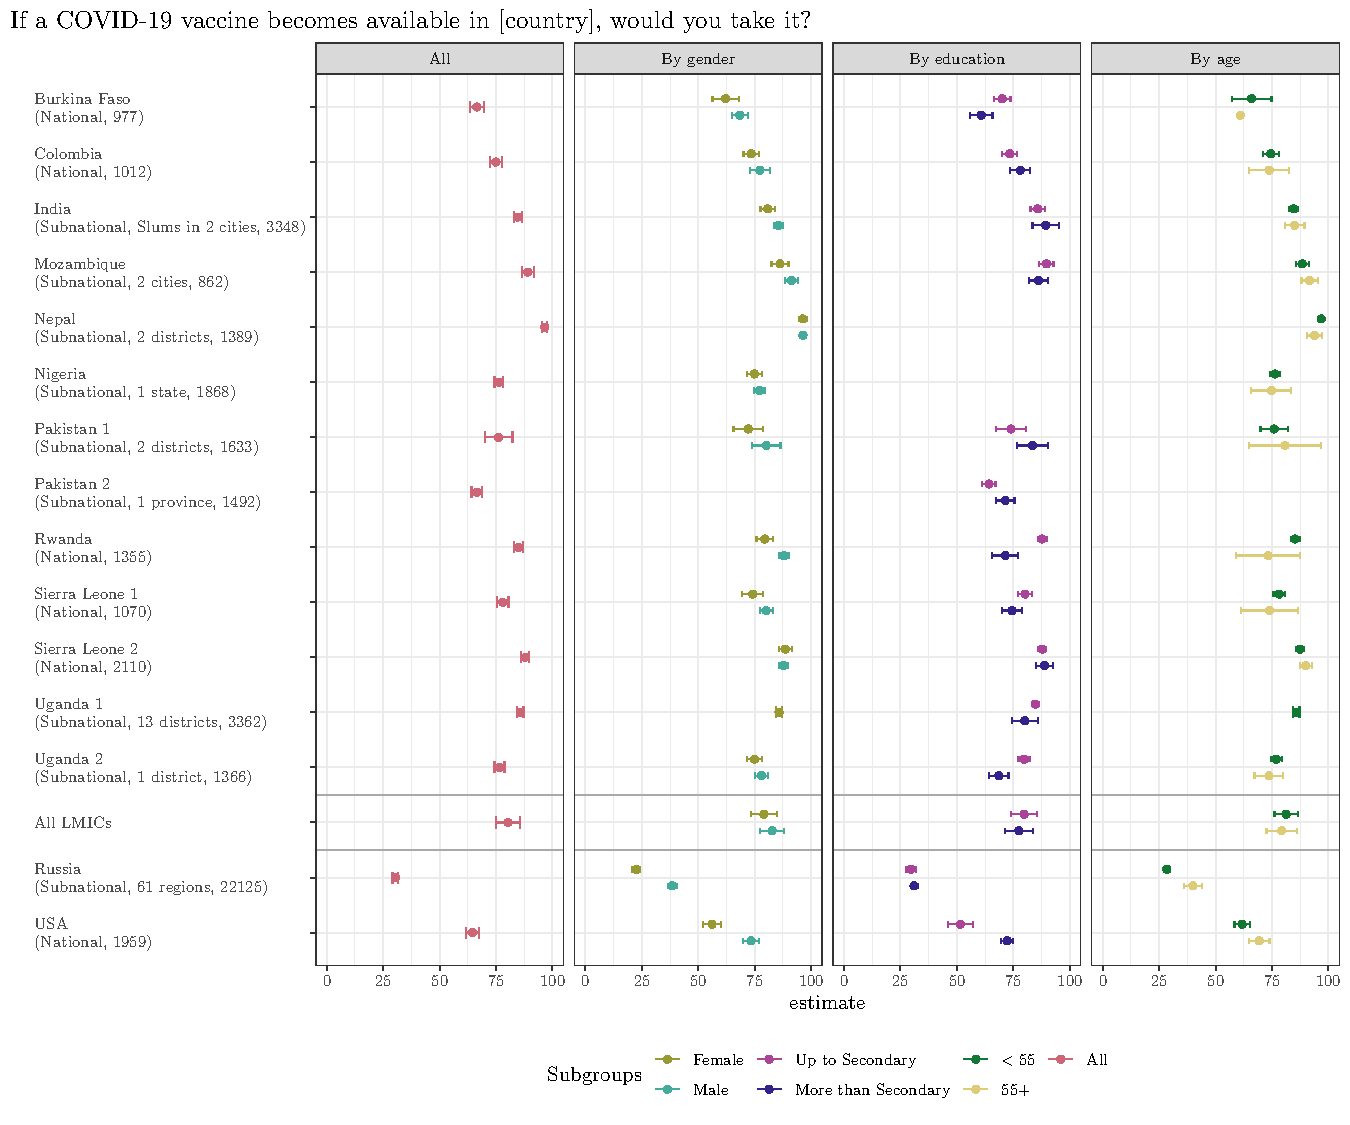
\includegraphics{paper_files/figure-latex/mainfigure1-1.pdf}

\scriptsize{Figure 1 presents average acceptance of the COVID-19 vaccine across studies and subgroups within studies. For each study, we summarize sampling information in parentheses in the following way: First, we indicate whether the geographic coverage of the sample is national or subnational. If the coverage is subnational we provide further details. Second, we list the number of observations included in the study. Data are presented as mean values +/- SD. In the plot, points represent the estimated percentage of individuals who would take the vaccine. ``No'', ``Don't know'' and ``Refuse'' are taken as a single reference category. Bars around each point indicate a 95\% confidence interval for the estimate. An estimate of average acceptance for all studies in LMICs (excluding USA and Russia) is also shown.}
\end{figure}

\begin{figure}[!ht]
\caption{Reasons not to take the vaccine \label{fig:fig2paper}}

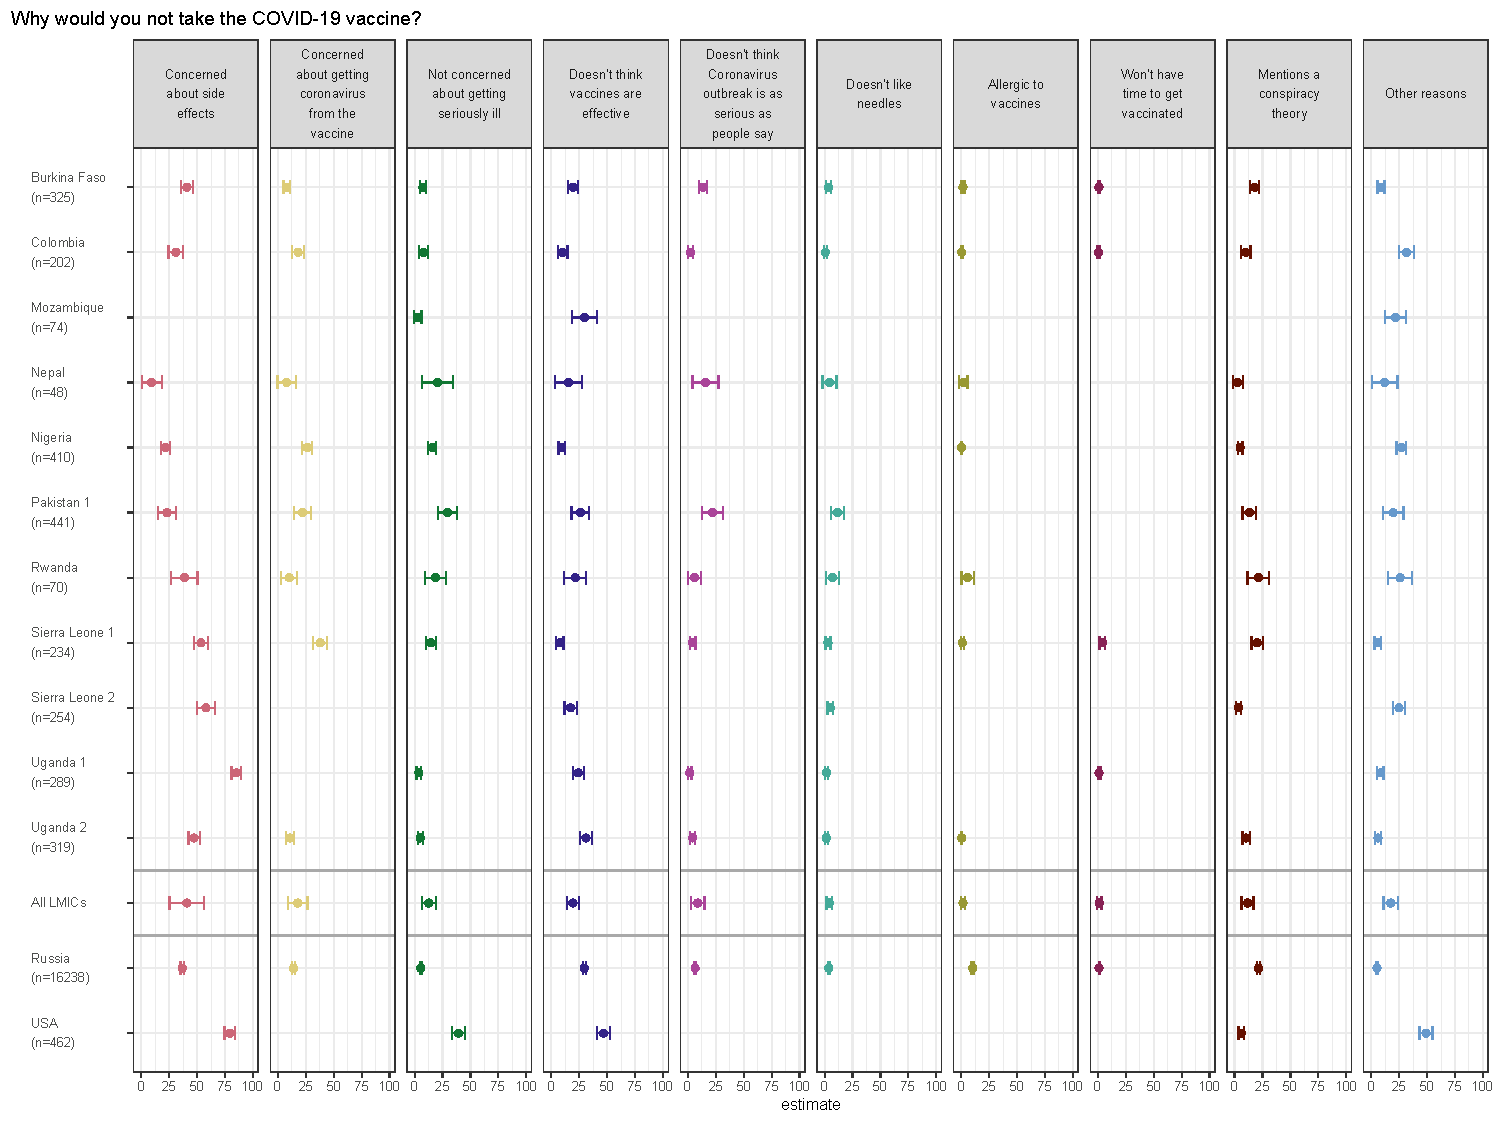
\includegraphics{paper_files/figure-latex/fig2paper-1.pdf}

\scriptsize{Figure 2 shows the percentage of respondents mentioning reasons why they would not take the COVID-19 vaccine. For each study, we present the sample size in parentheses. Data are presented as mean values +/- SD. In the plot, points represent the estimated percentage of individuals that would not take the vaccine or do not know if they would take the vaccine for each possible response option. Bars around each point indicate a 95\% confidence interval for the estimate. An estimated average for all studies in LMICs is also shown. Studies India and Pakistan 2 are not included because they either did not include the question or were not properly harmonized with the other studies.}
\end{figure}

\begin{figure}[!ht]
\caption{Trusted actors and institutions, broken down by expressed willingness to take a COVID-19 vaccine \label{fig:fig3paper}}

\newpage

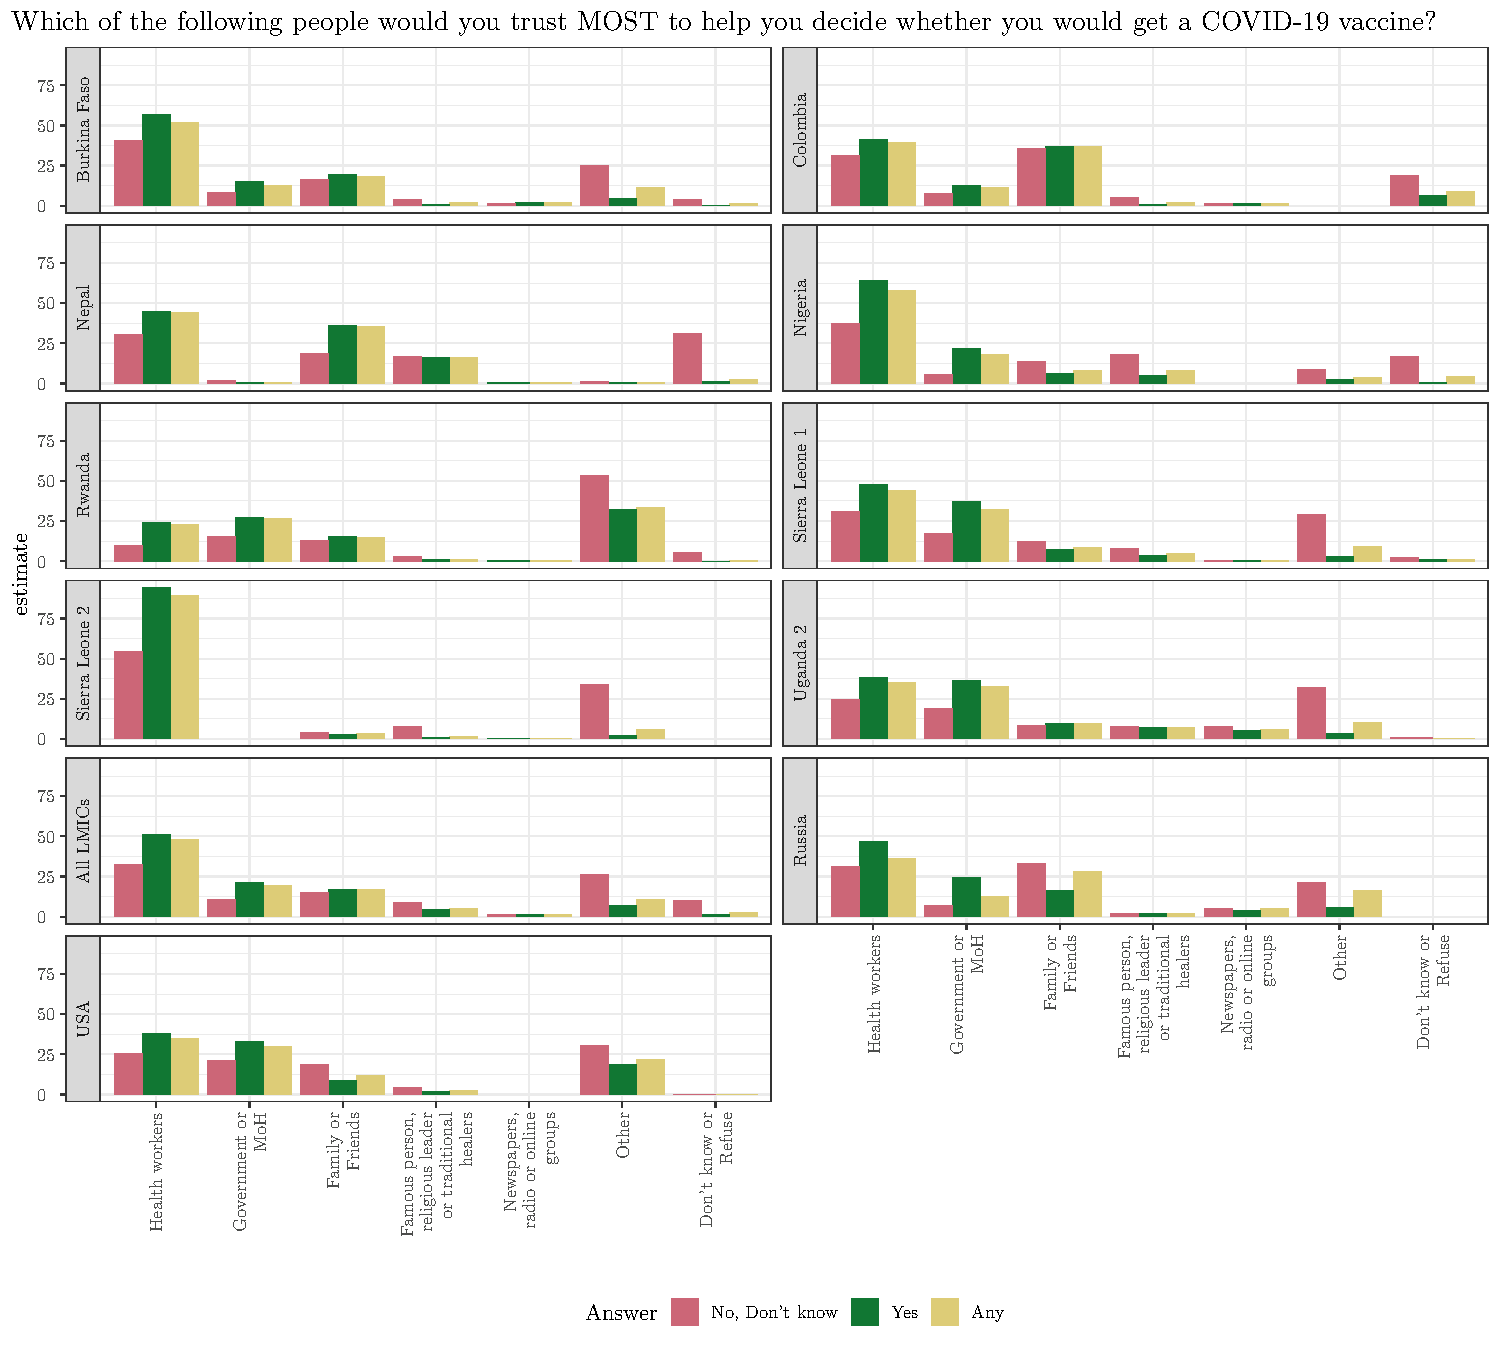
\includegraphics{paper_files/figure-latex/fig3paper-1.pdf}
\newpage

\scriptsize{Figure 3 shows histograms of actors and institutions respondents say they would trust most to help them decide whether to take the COVID-19 vaccine. Respondents were only permitted to select one most trusted actor or institution. Studies India, Mozambique, Pakistan 1, Pakistan 2 and Uganda 1 are not included because they either did not include the question or were not properly harmonized with the other studies.}
\end{figure}

\newpage

\begin{figure}[!ht]
\caption{Trusted actors and institutions, broken down by gender \label{fig:genderhist}}

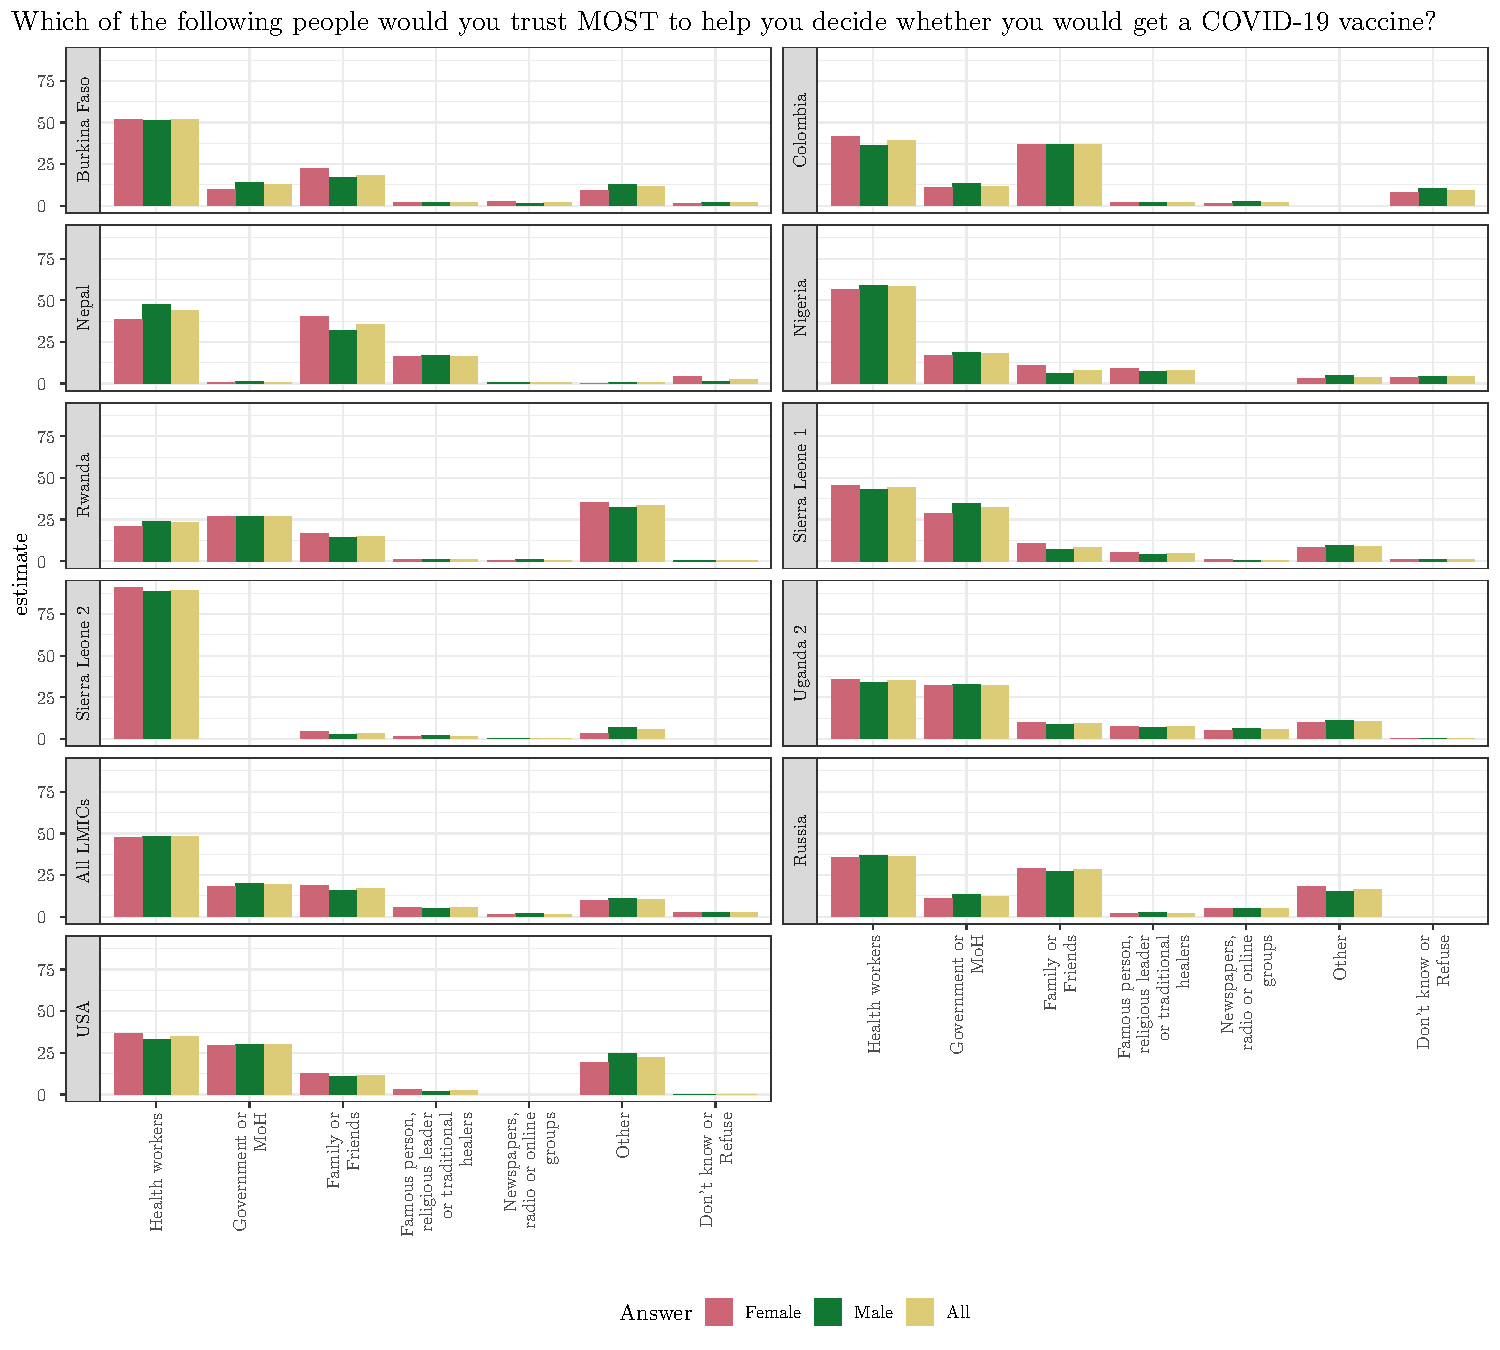
\includegraphics{paper_files/figure-latex/genderhist-1.pdf}

\scriptsize{Figure S1 shows histograms of actors and institutions that respondents say they would trust most to help them decide whether or not to take the COVID-19 vaccine. Respondents were only permitted to select one most trusted  actor or institution. Responses are broken down by gender of respondent.}
\end{figure}

\pagebreak

\begin{figure}[!ht]
\caption{Trusted actors and institutions, broken down by vaccine acceptance \label{fig:vaccacc}}

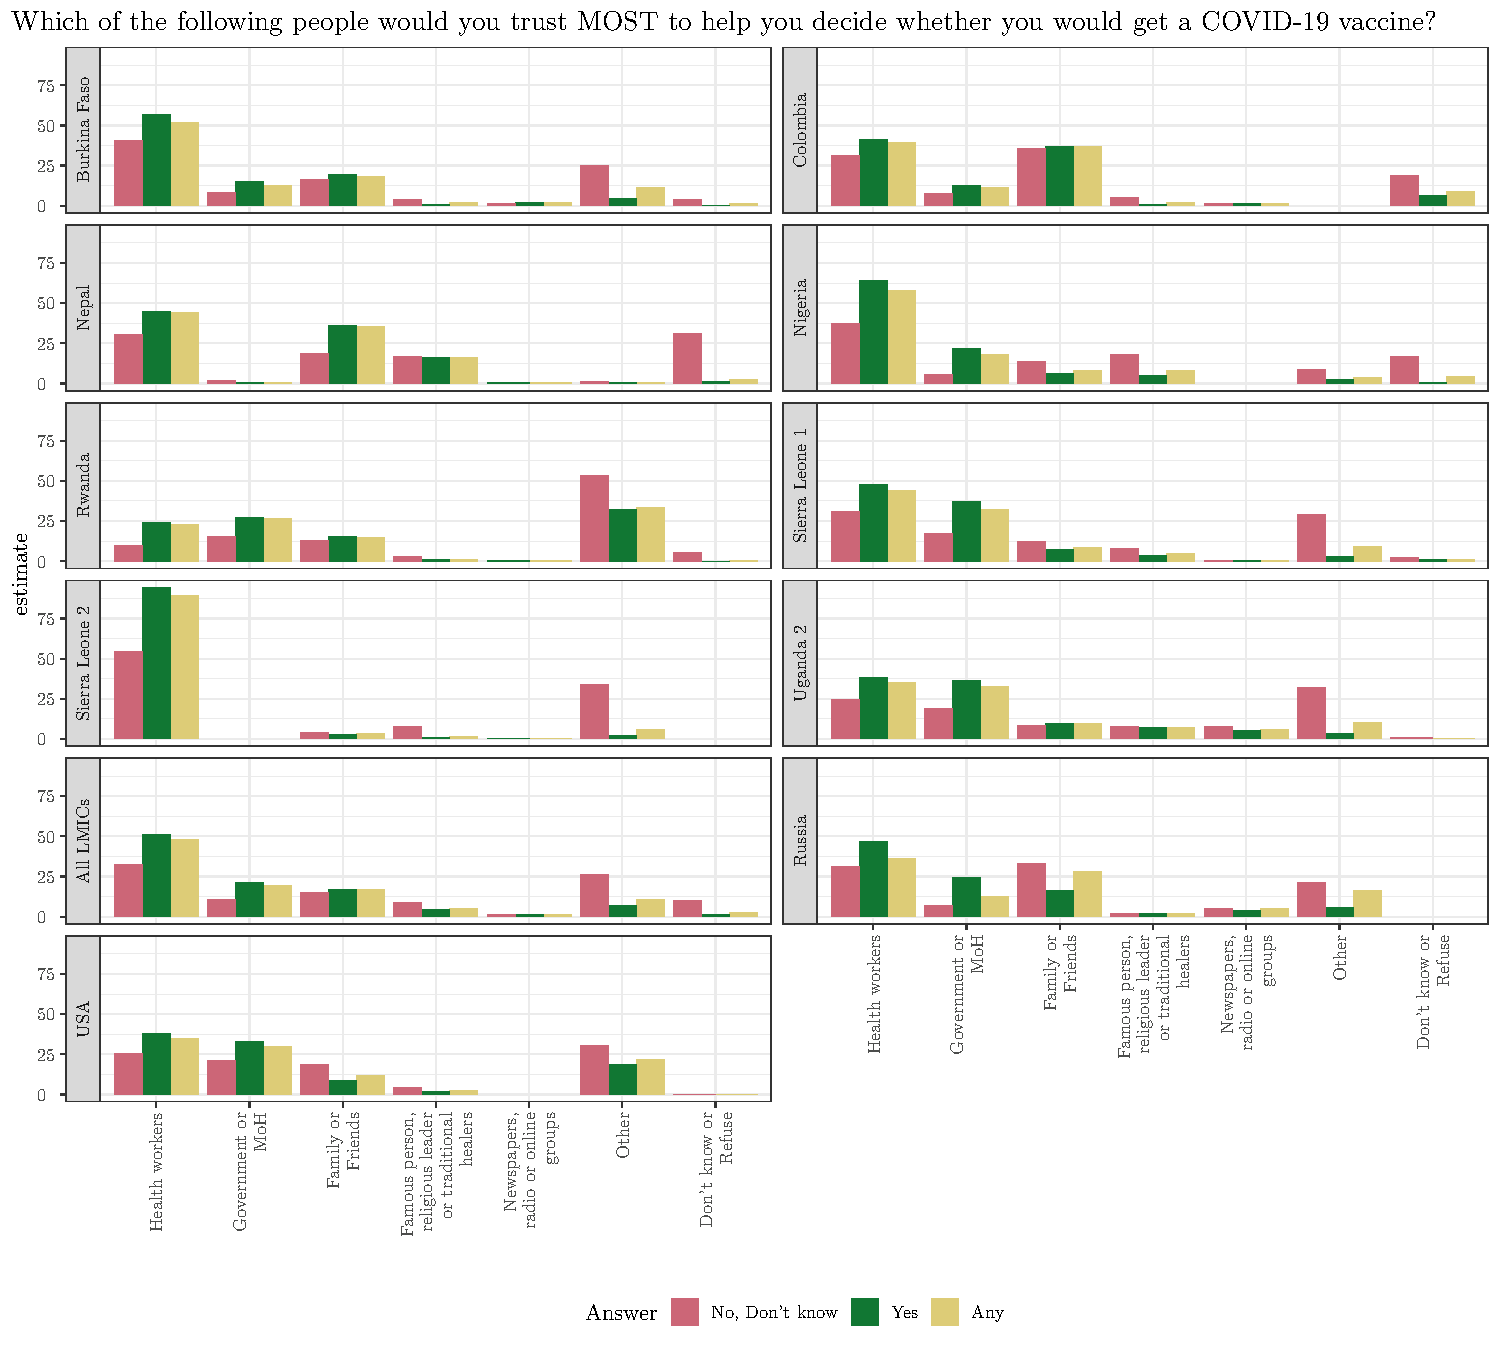
\includegraphics{paper_files/figure-latex/histcattrust-1.pdf}

\scriptsize{Figure S2 shows histograms of actors and institutions that respondents say they would trust most to help them decide whether or not to take the COVID-19 vaccine. Respondents were only permitted to select one most trusted  actor or institution. Responses are broken down by acceptance of the COVID-19 vaccine. The color of the bars reflect the answer given to the question ``If a COVID-19 vaccine becomes available in [country], would you take it?'' with ``No'' and ``Don't know'' pooled together and ``All'' combined average of ``Yes'' and ``No / Don't know''}
\end{figure}

\pagebreak

\begin{figure}[!ht]
\caption{Average vaccine acceptance across all LMIC countries leaving one or two study samples out
 \label{fig:mainloo}}

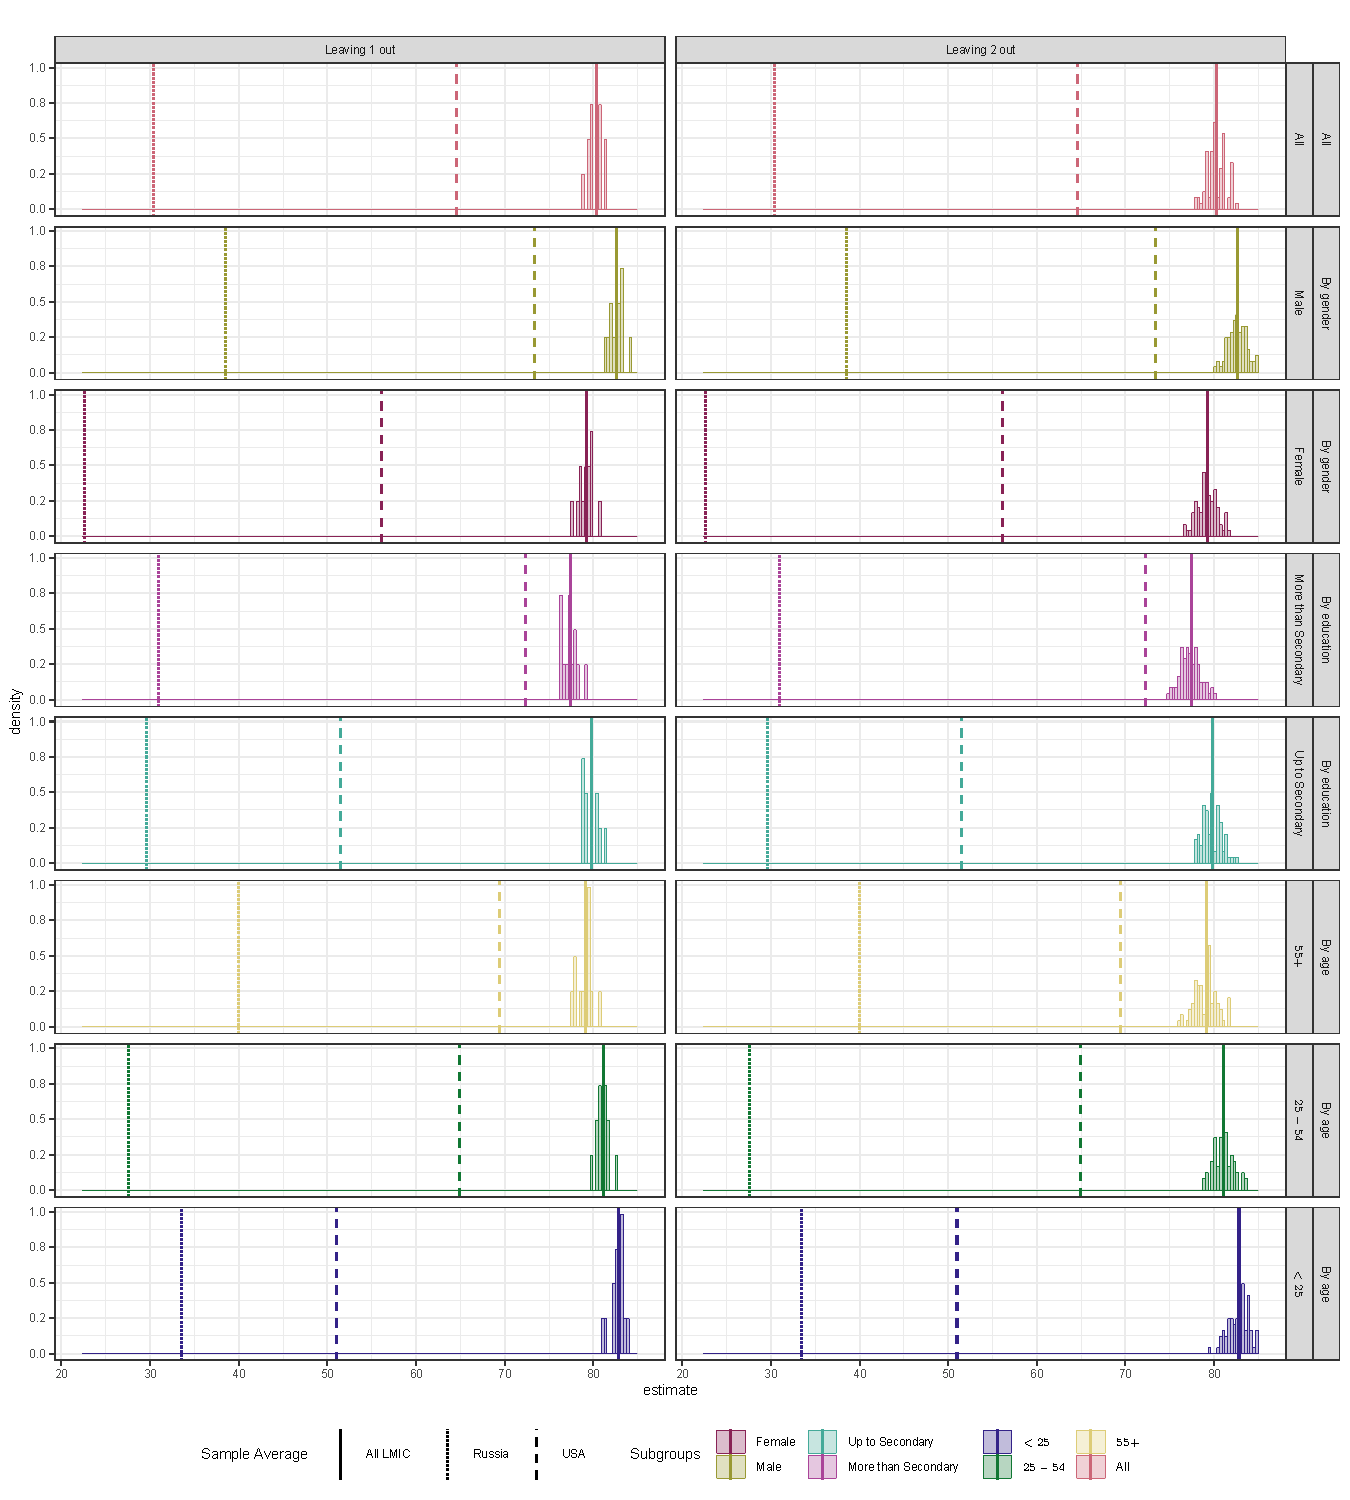
\includegraphics{paper_files/figure-latex/mainloo-1.pdf}

\scriptsize{Figure S3 shows distribution of estimates of average acceptance for all studies in LMICs (excluding USA and Russia) leaving one and two study samples out at a time. Figure also shows distributions of subgroup averages by gender, education and age leaving one and two study samples out at a time. To directly compare the resulting distributions to the estimates reported in Figure 1, we plot point estimates reported in Figure 1 for all LMIC studies, Russia and the US.}
\end{figure}

\pagebreak

\clearpage

\hypertarget{supplementary-appendix}{%
\section*{Supplementary Appendix}\label{supplementary-appendix}}
\addcontentsline{toc}{section}{Supplementary Appendix}

\setcounter{table}{0}  \renewcommand{\thetable}{S\arabic{table}} \setcounter{figure}{0} \renewcommand{\thefigure}{S\arabic{figure}}
\setcounter{page}{1}

\newpage

\begin{table}[!h]

\caption{\label{tab:maintabledis}If a COVID-19 vaccine becomes available in [country], would you take it? Disaggregated by subgroups}
\centering
\resizebox{\linewidth}{!}{
\fontsize{10}{12}\selectfont
\begin{threeparttable}
\begin{tabular}[t]{lcccccccc}
\toprule
\multicolumn{1}{c}{\textbf{}} & \multicolumn{1}{c}{\textbf{}} & \multicolumn{2}{c}{\textbf{Gender}} & \multicolumn{2}{c}{\textbf{Education}} & \multicolumn{3}{c}{\textbf{Age}} \\
\cmidrule(l{3pt}r{3pt}){3-4} \cmidrule(l{3pt}r{3pt}){5-6} \cmidrule(l{3pt}r{3pt}){7-9}
\textbf{Country} & \textbf{Average acceptability} & \textbf{Female} & \textbf{Male} & \textbf{> Secondary} & \textbf{Up to Secondary} & \textbf{<25} & \textbf{25-54} & \textbf{55+}\\
\midrule
Burkina Faso & 66.5 & 62.1 & 68.4 & 60.8 & 70.1 & 76.0 & 63.2 & .\\
 & (63.5, 69.5) & (56.3, 67.9) & (65.0, 71.9) & (55.9, 65.8) & (66.4, 73.8) & (58.0, 94.0) & (53.0, 73.4) & .\\
Colombia & 74.9 & 73.5 & 77.3 & 78.1 & 73.4 & 75.4 & 74.2 & 73.8\\
 & (72.2, 77.6) & (70.1, 77.0) & (73.0, 81.7) & (73.6, 82.5) & (70.1, 76.8) & (67.5, 83.4) & (70.2, 78.3) & (65.0, 82.6)\\
India & 84.3 & 82.4 & 84.7 & 87.8 & 85.9 & 77.6 & 85.4 & 83.1\\
 & (82.3, 86.3) & (79.0, 85.8) & (82.5, 87.0) & (81.1, 94.6) & (82.5, 89.2) & (71.6, 83.6) & (83.4, 87.3) & (77.6, 88.5)\\
Mozambique & 89.1 & 86.2 & 91.3 & 86.1 & 89.7 & . & 88.3 & 91.7\\
 & (86.5, 91.7) & (82.5, 90.0) & (88.4, 94.1) & (81.8, 90.4) & (86.5, 92.8) & . & (85.3, 91.2) & (88.1, 95.4)\\
Nepal & 96.6 & 96.4 & 96.4 & . & . & 97.8 & 96.6 & 93.8\\
 & (95.5, 97.6) & (94.6, 98.2) & (95.1, 97.7) & . & . & (95.7, 99.8) & (95.2, 97.9) & (90.4, 97.2)\\
Nigeria & 76.2 & 74.9 & 77.0 & . & . & 69.0 & 77.6 & 74.7\\
 & (74.3, 78.2) & (71.7, 78.1) & (74.6, 79.4) & . & . & (63.3, 74.7) & (75.5, 79.7) & (65.8, 83.6)\\
Pakistan 1 & 76.1 & 72.2 & 80.1 & 83.6 & 74.0 & 86.3 & 75.6 & 80.8\\
 & (70.0, 82.3) & (65.6, 78.8) & (73.8, 86.4) & (76.6, 90.5) & (67.4, 80.5) & (78.4, 94.1) & (69.3, 81.8) & (64.9, 96.7)\\
Pakistan 2 & 66.5 & . & . & 71.4 & 64.2 & . & . & .\\
 & (64.1, 68.9) & . & . & (67.3, 75.5) & (61.2, 67.1) & . & . & .\\
Rwanda & 84.9 & 79.4 & 88.0 & 71.4 & 87.7 & 88.1 & 83.8 & 73.3\\
 & (82.9, 86.8) & (75.8, 83.0) & (85.8, 90.2) & (65.5, 77.2) & (85.8, 89.7) & (85.0, 91.1) & (81.3, 86.3) & (59.2, 87.3)\\
Sierra Leone 1 & 78.0 & 74.1 & 80.1 & 74.4 & 80.2 & 78.0 & 78.3 & 74.0\\
 & (75.5, 80.5) & (69.5, 78.7) & (77.2, 83.1) & (70.1, 78.7) & (77.0, 83.3) & (72.4, 83.6) & (75.4, 81.1) & (61.4, 86.6)\\
Sierra Leone 2 & 87.9 & 88.6 & 87.7 & 88.8 & 87.8 & 82.9 & 87.6 & 90.0\\
 & (86.2, 89.6) & (85.7, 91.5) & (85.9, 89.5) & (85.0, 92.5) & (86.0, 89.6) & (73.9, 91.9) & (85.6, 89.5) & (87.4, 92.6)\\
Uganda 1 & 85.8 & 85.8 & . & 80.1 & 84.8 & 85.5 & 85.9 & .\\
 & (84.4, 87.2) & (84.4, 87.2) & . & (74.4, 85.9) & (83.2, 86.5) & (82.7, 88.4) & (84.3, 87.4) & .\\
Uganda 2 & 76.5 & 74.9 & 78.0 & 68.6 & 79.8 & 76.5 & 77.0 & 73.7\\
 & (74.3, 78.7) & (71.5, 78.3) & (75.2, 80.9) & (64.3, 72.9) & (77.3, 82.2) & (71.0, 82.1) & (74.4, 79.6) & (67.3, 80.0)\\
All LMICs & 80.3 & 79.2 & 82.6 & 77.4 & 79.8 & 82.8 & 81.1 & 79.1\\
 & (74.9, 85.6) & (73.4, 85.0) & (77.4, 87.9) & (71.4, 83.4) & (74.1, 85.4) & (76.9, 88.7) & (75.6, 86.6) & (72.5, 85.7)\\
All LMICs (National) & 78.4 & 75.5 & 80.3 & 74.7 & 79.8 & 80.1 & 77.4 & 74.4\\
 & (67.9, 89.0) & (63.6, 87.5) & (70.2, 90.4) & (62.1, 87.3) & (69.8, 89.9) & (73.4, 86.7) & (65.7, 89.2) & (61.7, 87.2)\\
Russia & 30.4 & 22.6 & 38.5 & 31.0 & 29.6 & 33.5 & 27.6 & 40.0\\
 & (29.1, 31.7) & (20.9, 24.2) & (36.5, 40.5) & (29.6, 32.5) & (27.3, 32.0) & (29.2, 37.7) & (26.2, 28.9) & (35.9, 44.0)\\
USA & 64.6 & 56.1 & 73.4 & 72.3 & 51.5 & 51.0 & 64.9 & 69.4\\
 & (61.8, 67.3) & (52.1, 60.1) & (69.8, 76.9) & (69.5, 75.0) & (46.0, 57.0) & (43.5, 58.6) & (61.1, 68.7) & (64.8, 73.9)\\
\bottomrule
\end{tabular}
\begin{tablenotes}
\item Table S1 shows percentage of respondents willing to take the COVID-19 vaccine as plotted in Figure 1. A 95\% confidence interval is shown between parentheses.
\end{tablenotes}
\end{threeparttable}}
\end{table}

\newpage

\begin{table}

\caption{\label{tab:yes}Reasons to take the vaccine}
\centering
\fontsize{10}{12}\selectfont
\begin{threeparttable}
\begin{tabular}[t]{>{\raggedright\arraybackslash}p{8em}>{\centering\arraybackslash}p{4em}>{\centering\arraybackslash}p{4em}>{\centering\arraybackslash}p{4em}c}
\toprule
\multicolumn{2}{c}{\textbf{ }} & \multicolumn{3}{c}{\textbf{Protection}} \\
\cmidrule(l{3pt}r{3pt}){3-5}
\textbf{Study} & \textbf{N} & \textbf{Self} & \textbf{Family} & \textbf{Community}\\
\midrule
Burkina Faso & 651 & 76 & 42 & 7\\
 &  & (73, 79) & (38, 46) & (5, 9)\\
Colombia & 756 & 91 & 23 & 12\\
 &  & (88, 93) & (20, 26) & (10, 14)\\
Mozambique & 768 & 83 & 32 & 4\\
 &  & (80, 86) & (27, 38) & (2, 5)\\
Nepal & 1341 & 96 & 34 & 20\\
 &  & (95, 98) & (32, 37) & (17, 22)\\
Nigeria & 1424 & 89 & 35 & 21\\
 &  & (88, 91) & (33, 38) & (19, 23)\\
Rwanda & 1152 & 98 & 26 & 11\\
 &  & (97, 99) & (23, 28) & (9, 13)\\
Sierra Leone 1 & 836 & 94 & 37 & 21\\
 &  & (92, 96) & (34, 40) & (18, 23)\\
Sierra Leone 2 & 1855 & 91 & 62 & 21\\
 &  & (88, 93) & (57, 66) & (16, 27)\\
Uganda 1 & 2885 & 96 & 36 & 9\\
 &  & (95, 97) & (34, 38) & (8, 10)\\
Uganda 2 & 1045 & 96 & 28 & 11\\
 &  & (95, 97) & (25, 31) & (9, 12)\\
All LMICs & . & 91 & 36 & 14\\
 &  & (86, 96) & (28, 43) & (9, 18)\\
Russia & 5887 & 76 & 69 & 41\\
 &  & (74, 78) & (67, 71) & (38, 43)\\
USA & 1313 & 94 & 92 & 89\\
 &  & (92, 95) & (90, 94) & (87, 91)\\
\bottomrule
\end{tabular}
\begin{tablenotes}
\item Table S2 shows percentage of respondents mentioning reasons why they would take the Covid-19 vaccine. The number of observations and percentage corresponds only to people who would take the vaccine. Respondents in all countries could give more than one reason. A 95\% confidence interval is shown between parentheses. Studies India, Pakistan 1 and Pakistan 2 are not included because they either did not include the question or were not properly harmonized with the other studies.
\end{tablenotes}
\end{threeparttable}
\end{table}

\newpage

\begin{table}[!h]

\caption{\label{tab:yesall}Reasons to take the vaccine- all categories}
\centering
\resizebox{\linewidth}{!}{
\fontsize{10}{12}\selectfont
\begin{threeparttable}
\begin{tabular}[t]{>{\raggedright\arraybackslash}p{7em}>{\centering\arraybackslash}p{7em}>{\centering\arraybackslash}p{7em}>{\centering\arraybackslash}p{7em}>{\centering\arraybackslash}p{7em}>{\centering\arraybackslash}p{7em}>{\centering\arraybackslash}p{7em}>{\centering\arraybackslash}p{7em}}
\toprule
\multicolumn{2}{c}{\textbf{ }} & \multicolumn{3}{c}{\textbf{Protection}} & \multicolumn{2}{c}{\textbf{If recommended by}} & \multicolumn{1}{c}{\textbf{ }} \\
\cmidrule(l{3pt}r{3pt}){3-5} \cmidrule(l{3pt}r{3pt}){6-7}
\textbf{Study} & \textbf{N} & \textbf{Self} & \textbf{Family} & \textbf{Community} & \textbf{Health workers} & \textbf{Government} & \textbf{Other}\\
\midrule
Burkina Faso & 651 & 76 & 42 & 7 & 6 & 19 & 2\\
 &  & (73, 79) & (38, 46) & (5, 9) & (4, 8) & (16, 22) & (1, 3)\\
Colombia & 756 & 91 & 23 & 12 & 1 & 2 & 6\\
 &  & (88, 93) & (20, 26) & (10, 14) & (0, 2) & (1, 3) & (4, 7)\\
Mozambique & 768 & 83 & 32 & 4 & . & 7 & 3\\
 &  & (80, 86) & (27, 38) & (2, 5) & . & (5, 8) & (2, 4)\\
Nepal & 1341 & 96 & 34 & 20 & 2 & 3 & 7\\
 &  & (95, 98) & (32, 37) & (17, 22) & (1, 2) & (2, 4) & (5, 9)\\
Nigeria & 1424 & 89 & 35 & 21 & . & 6 & 4\\
 &  & (88, 91) & (33, 38) & (19, 23) & . & (4, 7) & (3, 5)\\
Rwanda & 1152 & 98 & 26 & 11 & 1 & 5 & 1\\
 &  & (97, 99) & (23, 28) & (9, 13) & (0, 1) & (4, 6) & (1, 2)\\
Sierra Leone 1 & 836 & 94 & 37 & 21 & 12 & 23 & 7\\
 &  & (92, 96) & (34, 40) & (18, 23) & (10, 14) & (20, 25) & (5, 9)\\
Sierra Leone 2 & 1855 & 91 & 62 & 21 & 59 & . & 16\\
 &  & (88, 93) & (57, 66) & (16, 27) & (54, 63) & . & (11, 21)\\
Uganda 1 & 2885 & 96 & 36 & 9 & . & 10 & 6\\
 &  & (95, 97) & (34, 38) & (8, 10) & . & (9, 12) & (5, 7)\\
Uganda 2 & 1045 & 96 & 28 & 11 & 1 & 15 & 2\\
 &  & (95, 97) & (25, 31) & (9, 12) & (1, 2) & (13, 17) & (1, 3)\\
All LMICs & . & 91 & 36 & 14 & 12 & 10 & 5\\
 &  & (86, 96) & (28, 43) & (9, 18) & (-8, 31) & (4, 16) & (2, 8)\\
Russia & 5887 & 76 & 69 & 41 & 11 & 6 & 18\\
 &  & (74, 78) & (67, 71) & (38, 43) & (10, 13) & (5, 7) & (16, 20)\\
USA & 1313 & 94 & 92 & 89 & . & 67 & .\\
 &  & (92, 95) & (90, 94) & (87, 91) & . & (64, 70) & .\\
\bottomrule
\end{tabular}
\begin{tablenotes}
\item Table S3 shows percentage of respondents mentioning reasons why they would take the Covid-19 vaccine. The number of observations and percentage correponds only to people who would take the vaccine. Respondents in all countries could give more than one reason. A 95\% confidence interval is shown between parentheses.
\end{tablenotes}
\end{threeparttable}}
\end{table}

\newpage

\begin{table}[!h]

\caption{\label{tab:yes1}Reasons to take the vaccine- by age groups}
\centering
\resizebox{\linewidth}{!}{
\fontsize{10}{12}\selectfont
\begin{threeparttable}
\begin{tabular}[t]{>{\raggedright\arraybackslash}p{7em}>{\centering\arraybackslash}p{5em}>{\centering\arraybackslash}p{5em}>{\centering\arraybackslash}p{5em}>{\centering\arraybackslash}p{5em}>{\centering\arraybackslash}p{5em}>{\centering\arraybackslash}p{5em}>{\centering\arraybackslash}p{5em}>{\centering\arraybackslash}p{5em}>{\centering\arraybackslash}p{5em}}
\toprule
\multicolumn{1}{c}{\textbf{ }} & \multicolumn{3}{c}{\textbf{Self}} & \multicolumn{3}{c}{\textbf{Family}} & \multicolumn{3}{c}{\textbf{Community}} \\
\cmidrule(l{3pt}r{3pt}){2-4} \cmidrule(l{3pt}r{3pt}){5-7} \cmidrule(l{3pt}r{3pt}){8-10}
\textbf{Study} & \textbf{<25} & \textbf{25-54} & \textbf{55+} & \textbf{<25} & \textbf{25-54} & \textbf{55+} & \textbf{<25} & \textbf{25-54} & \textbf{55+}\\
\midrule
Burkina Faso & 77 & 59 & 100 & 26 & 64 & 66 & 11 & 2 & 0\\
Conf. interval & (56, 99) & (46, 72) & (100, 100) & (4, 48) & (51, 77) & (-80, 211) & (-5, 26) & (-2, 5) & (0, 0)\\
n & 19 & 57 & 3 & 19 & 57 & 3 & 19 & 57 & 3\\
\midrule
Colombia & 91 & 91 & 90 & 26 & 26 & 16 & 12 & 13 & 14\\
Conf. interval & (86, 97) & (88, 94) & (83, 97) & (17, 35) & (21, 31) & (8, 25) & (4, 20) & (9, 16) & (6, 22)\\
n & 90 & 349 & 73 & 90 & 349 & 73 & 90 & 349 & 73\\
\midrule
Mozambique & 62 & 84 & 80 & 50 & 32 & 34 & 12 & 4 & 2\\
Conf. interval & (19, 106) & (81, 87) & (75, 86) & (5, 95) & (26, 38) & (27, 41) & (-17, 42) & (2, 6) & (0, 4)\\
n & 8 & 571 & 188 & 8 & 571 & 188 & 8 & 571 & 188\\
\midrule
Nepal & 97 & 97 & 92 & 31 & 36 & 27 & 15 & 20 & 19\\
Conf. interval & (94, 100) & (96, 98) & (87, 97) & (25, 37) & (33, 39) & (19, 36) & (10, 20) & (17, 23) & (13, 25)\\
n & 225 & 890 & 162 & 225 & 890 & 162 & 225 & 890 & 162\\
\midrule
Nigeria & 91 & 89 & 94 & 31 & 36 & 31 & 22 & 21 & 21\\
Conf. interval & (87, 95) & (87, 91) & (89, 100) & (25, 38) & (33, 39) & (20, 42) & (16, 29) & (18, 23) & (11, 31)\\
n & 178 & 1175 & 71 & 178 & 1175 & 71 & 178 & 1175 & 71\\
\midrule
Rwanda & 98 & 98 & 100 & 22 & 28 & 29 & 10 & 11 & 10\\
Conf. interval & (97, 100) & (97, 99) & (100, 100) & (17, 26) & (24, 31) & (12, 46) & (7, 13) & (9, 14) & (-1, 21)\\
n & 389 & 732 & 31 & 389 & 732 & 31 & 389 & 732 & 31\\
\midrule
Sierra Leone 1 & 96 & 94 & 94 & 36 & 38 & 27 & 24 & 20 & 22\\
Conf. interval & (93, 99) & (92, 95) & (86, 102) & (29, 44) & (34, 41) & (12, 42) & (17, 31) & (16, 23) & (8, 36)\\
n & 167 & 632 & 37 & 167 & 632 & 37 & 167 & 632 & 37\\
\midrule
Sierra Leone 2 & 87 & 90 & 93 & 52 & 62 & 62 & 29 & 22 & 18\\
Conf. interval & (78, 97) & (88, 92) & (89, 97) & (39, 66) & (58, 67) & (56, 67) & (16, 42) & (16, 28) & (12, 25)\\
n & 63 & 1376 & 396 & 63 & 1376 & 396 & 63 & 1376 & 396\\
\midrule
Uganda 1 & 96 & 96 & . & 34 & 36 & . & 9 & 9 & .\\
Conf. interval & (95, 98) & (96, 97) & . & (30, 39) & (34, 39) & . & (6, 11) & (8, 11) & .\\
n & 526 & 2218 & . & 526 & 2218 & . & 526 & 2218 & .\\
\midrule
Uganda 2 & 97 & 96 & 97 & 20 & 30 & 28 & 8 & 11 & 13\\
Conf. interval & (94, 99) & (95, 97) & (94, 100) & (14, 26) & (27, 33) & (21, 36) & (4, 11) & (9, 13) & (7, 19)\\
n & 173 & 749 & 123 & 173 & 749 & 123 & 173 & 749 & 123\\
\midrule
All LMICs & 89 & 89 & 93 & 33 & 39 & 36 & 15 & 13 & 13\\
Conf. interval & (81, 97) & (81, 98) & (89, 98) & (25, 41) & (29, 48) & (23, 48) & (10, 20) & (8, 18) & (7, 19)\\
n & 1838 & 8749 & 1084 & 1838 & 8749 & 1084 & 1838 & 8749 & 1084\\
\midrule
Russia & 67 & 76 & 81 & 74 & 68 & 68 & 46 & 40 & 38\\
Conf. interval & (59, 74) & (73, 78) & (76, 87) & (68, 81) & (66, 71) & (62, 74) & (38, 54) & (38, 43) & (32, 44)\\
n & 552 & 5108 & 227 & 552 & 5108 & 227 & 552 & 5108 & 227\\
\midrule
USA & 92 & 91 & 97 & 89 & 91 & 94 & 90 & 89 & 89\\
Conf. interval & (88, 96) & (89, 94) & (95, 99) & (83, 95) & (88, 93) & (91, 97) & (85, 95) & (86, 92) & (85, 93)\\
n & 153 & 687 & 473 & 153 & 687 & 473 & 153 & 687 & 473\\
\bottomrule
\end{tabular}
\begin{tablenotes}
\item Table S4 shows percentage of respondents mentioning reasons why they would take the Covid-19 vaccine by age groups. The number of observations and percentage correponds only to people who would take the vaccine. Respondents in all countries could give more than one reason. A 95\% confidence interval is shown between parentheses.
\end{tablenotes}
\end{threeparttable}}
\end{table}

\newpage

\begin{landscape}\begin{table}[!h]

\caption{\label{tab:no}Reasons not to take the vaccine}
\centering
\resizebox{\linewidth}{!}{
\fontsize{10}{12}\selectfont
\begin{threeparttable}
\begin{tabular}[t]{>{\raggedright\arraybackslash}p{7em}>{\centering\arraybackslash}p{7em}>{\centering\arraybackslash}p{7em}>{\centering\arraybackslash}p{7em}>{\centering\arraybackslash}p{7em}>{\centering\arraybackslash}p{7em}>{\centering\arraybackslash}p{7em}>{\centering\arraybackslash}p{7em}>{\centering\arraybackslash}p{7em}>{\centering\arraybackslash}p{7em}>{\centering\arraybackslash}p{7em}>{\centering\arraybackslash}p{7em}}
\toprule
\textbf{Study} & \textbf{N} & \textbf{Concerned about side effects} & \textbf{Concerned about getting coronavirus from the vaccine} & \textbf{Not concerned about getting seriously ill} & \textbf{Doesn't think vaccines are effective} & \textbf{Doesn't think Coronavirus outbreak is as serious as people say} & \textbf{Doesn't like needles} & \textbf{Allergic to vaccines} & \textbf{Won't have time to get vaccinated} & \textbf{Mentions a conspiracy theory} & \textbf{Other reasons}\\
\midrule
Burkina Faso & 325 & 40.9 & 8.0 & 7.4 & 19.5 & 13.5 & 3.5 & 1.5 & 0.9 & 17.9 & 8.7\\
 &  & (35.5, 46.3) & ( 5.0, 11.0) & ( 4.5, 10.2) & (15.1, 23.8) & ( 9.8, 17.2) & ( 1.5,  5.6) & ( 0.2,  2.8) & (-0.1,  1.9) & (13.7, 22.1) & ( 5.6, 11.8)\\
Colombia & 202 & 31.0 & 18.1 & 8.0 & 10.2 & 2.3 & 0.6 & 0.4 & 0.5 & 10.0 & 31.6\\
 &  & (24.4, 37.6) & (12.7, 23.4) & ( 3.9, 12.0) & ( 5.9, 14.5) & ( 0.3,  4.3) & (-0.6,  1.8) & (-0.4,  1.3) & (-0.5,  1.5) & ( 5.8, 14.2) & (25.1, 38.2)\\
Mozambique & 74 & . & . & 2.7 & 29.7 & . & . & . & . & . & 21.6\\
 &  & . & . & (-0.7,  6.1) & (18.6, 40.8) & . & . & . & . & . & (12.2, 31.0)\\
Nepal & 48 & 9.3 & 7.9 & 20.4 & 15.2 & 15.7 & 4.4 & 1.8 & . & 2.8 & 12.1\\
 &  & ( 0.3, 18.2) & (-0.4, 16.3) & ( 6.7, 34.1) & ( 3.2, 27.2) & ( 4.0, 27.3) & (-1.9, 10.6) & (-1.9,  5.5) & . & (-1.5,  7.2) & ( 0.8, 23.5)\\
Nigeria & 410 & 21.5 & 26.1 & 15.9 & 9.3 & . & . & 0.2 & . & 4.9 & 26.8\\
 &  & (17.5, 25.5) & (21.8, 30.4) & (12.3, 19.4) & ( 6.4, 12.1) & . & . & (-0.2,  0.7) & . & ( 2.8,  7.0) & (22.5, 31.1)\\
Pakistan 1 & 441 & 23.0 & 21.9 & 29.4 & 26.0 & 22.1 & 11.5 & . & . & 13.2 & 19.6\\
 &  & (15.1, 30.8) & (14.3, 29.4) & (20.9, 37.9) & (18.0, 34.0) & (12.8, 31.3) & ( 5.5, 17.4) & . & . & ( 7.1, 19.4) & (10.4, 28.8)\\
Rwanda & 70 & 38.6 & 10.1 & 18.7 & 21.5 & 5.8 & 7.0 & 5.6 & . & 21.3 & 25.8\\
 &  & (26.9, 50.3) & ( 2.8, 17.3) & ( 9.3, 28.1) & (11.6, 31.4) & ( 0.1, 11.4) & ( 0.9, 13.2) & ( 0.1, 11.1) & . & (11.5, 31.1) & (15.3, 36.3)\\
Sierra Leone 1 & 234 & 53.5 & 37.9 & 14.6 & 7.5 & 4.2 & 3.0 & 0.9 & 4.0 & 20.3 & 5.7\\
 &  & (47.1, 59.9) & (31.6, 44.2) & (10.1, 19.2) & ( 4.2, 10.9) & ( 1.6,  6.8) & ( 0.8,  5.2) & (-0.4,  2.2) & ( 1.4,  6.5) & (15.1, 25.5) & ( 2.8,  8.7)\\
Sierra Leone 2 & 254 & 57.9 & . & . & 17.3 & . & 5.1 & . & 0.0 & 3.5 & 24.8\\
 &  & (50.1, 65.7) & . & . & (11.9, 22.7) & . & ( 2.5,  7.8) & . & ( 0.0,  0.0) & ( 1.3,  5.7) & (19.3, 30.3)\\
Uganda 1 & 289 & 85.1 & . & 3.8 & 24.2 & 1.7 & 1.7 & . & 1.0 & . & 8.0\\
 &  & (80.7, 89.6) & . & ( 1.7,  5.9) & (19.2, 29.2) & ( 0.2,  3.2) & ( 0.2,  3.2) & . & (-0.1,  2.2) & . & ( 4.9, 11.0)\\
Uganda 2 & 319 & 47.3 & 10.7 & 5.0 & 31.0 & 4.1 & 1.6 & 0.3 & . & 10.3 & 6.0\\
 &  & (42.2, 52.5) & ( 7.1, 14.2) & ( 2.7,  7.3) & (25.9, 36.2) & ( 1.9,  6.2) & ( 0.2,  2.9) & (-0.3,  0.9) & . & ( 7.0, 13.7) & ( 3.4,  8.5)\\
All LMICs & . & 40.8 & 17.6 & 12.6 & 19.2 & 8.7 & 4.3 & 1.5 & 1.3 & 11.6 & 17.3\\
 &  & (25.3, 56.3) & ( 8.7, 26.5) & ( 6.4, 18.8) & (13.8, 24.7) & ( 2.4, 14.9) & ( 1.7,  6.8) & (-0.2,  3.3) & (-0.6,  3.2) & ( 6.1, 17.0) & (11.0, 23.7)\\
Russia & 16238 & 36.8 & 13.9 & 5.4 & 29.6 & 6.4 & 3.7 & 10.2 & 1.0 & 21.4 & 5.1\\
 &  & (35.2, 38.4) & (12.8, 15.1) & ( 4.6,  6.1) & (28.1, 31.1) & ( 5.6,  7.3) & ( 3.1,  4.3) & ( 9.2, 11.2) & ( 0.7,  1.4) & (20.1, 22.8) & ( 4.4,  5.8)\\
USA & 462 & 79.3 & . & 39.3 & 46.8 & . & . & . & . & 6.0 & 49.1\\
 &  & (74.6, 84.0) & . & (33.5, 45.0) & (41.0, 52.6) & . & . & . & . & ( 3.4,  8.7) & (43.3, 54.9)\\
\bottomrule
\end{tabular}
\begin{tablenotes}
\item Table S5 shows percentage of respondents mentioning reasons why they would not take the Covid-19 vaccine. The number of observations and percentage correponds only to people who would NOT take the vaccine. Respondents in all countries could give more than one reason. A 95\% confidence interval is shown between parentheses.
\end{tablenotes}
\end{threeparttable}}
\end{table}
\end{landscape}

\newpage

\begin{landscape}\begingroup\fontsize{10}{12}\selectfont

\begin{ThreePartTable}
\begin{TableNotes}
\item Table S6 shows percentage of respondents that mention actors who they would trust the most to help them decide whether to get a COVID-19 vaccine. For all countries the questions was asked regardless if respondent would take a vaccine, would not take it, does not know or does not respond. For India respondents were able to mention more than one actor, for the rest of countries only one actor was allowed. While rows should sum to 100\%, rounding makes number slightly above or below. A 95\% confidence interval is shown between parentheses.
\end{TableNotes}
\begin{longtable}[t]{>{\raggedright\arraybackslash}p{7em}>{\centering\arraybackslash}p{4em}>{\centering\arraybackslash}p{4em}>{\centering\arraybackslash}p{6em}>{\centering\arraybackslash}p{6em}>{\centering\arraybackslash}p{6em}>{\centering\arraybackslash}p{6em}>{\centering\arraybackslash}p{6em}>{\centering\arraybackslash}p{6em}>{\centering\arraybackslash}p{6em}}
\caption{\label{tab:trust}COVID-19 Vaccination Decision-making: most trusted source}\\
\toprule
\textbf{Study} & \textbf{N} & \textbf{Take vaccine?} & \textbf{Health workers} & \textbf{Government or Ministry of Health} & \textbf{Family or friends} & \textbf{Famous person, religious leader or traditional healers} & \textbf{Newspapers, radio or online groups} & \textbf{Other} & \textbf{Don't know or Refuse}\\
\midrule
\endfirsthead
\caption[]{\label{tab:trust}COVID-19 Vaccination Decision-making: most trusted source \textit{(continued)}}\\
\toprule
\textbf{Study} & \textbf{N} & \textbf{Take vaccine?} & \textbf{Health workers} & \textbf{Government or Ministry of Health} & \textbf{Family or friends} & \textbf{Famous person, religious leader or traditional healers} & \textbf{Newspapers, radio or online groups} & \textbf{Other} & \textbf{Don't know or Refuse}\\
\midrule
\endhead

\endfoot
\bottomrule
\insertTableNotes
\endlastfoot
Burkina Faso & 651 & Yes & 57.1 & 15.1 & 19.6 & 0.9 & 2.0 & 4.8 & 0.4\\
 &  &  & (53.3, 60.9) & (12.4, 17.9) & (16.5, 22.7) & ( 0.2,  1.6) & ( 0.9,  3.1) & ( 3.2,  6.4) & (-0.1,  0.9)\\
Burkina Faso & 325 & No & 40.7 & 8.5 & 16.2 & 3.7 & 1.6 & 25.1 & 4.2\\
 &  &  & (35.3, 46.1) & ( 5.5, 11.6) & (12.1, 20.2) & ( 1.6,  5.7) & ( 0.2,  3.0) & (20.3, 29.8) & ( 2.0,  6.4)\\
Burkina Faso & 976 & All & 51.6 & 12.9 & 18.4 & 1.8 & 1.9 & 11.6 & 1.7\\
 &  &  & (48.5, 54.8) & (10.8, 15.0) & (16.0, 20.9) & ( 1.0,  2.7) & ( 1.0,  2.7) & ( 9.6, 13.6) & ( 0.9,  2.5)\\
Colombia & 756 & Yes & 41.4 & 12.7 & 36.9 & 0.9 & 1.7 & . & 6.3\\
 &  &  & (37.8, 45.0) & (10.3, 15.2) & (33.4, 40.4) & ( 0.2,  1.5) & ( 0.8,  2.7) & . & ( 4.6,  8.1)\\
Colombia & 202 & No & 31.5 & 7.6 & 35.5 & 5.3 & 1.4 & . & 18.8\\
 &  &  & (24.9, 38.1) & ( 3.8, 11.3) & (28.8, 42.1) & ( 2.2,  8.4) & (-0.2,  3.0) & . & (13.2, 24.3)\\
Colombia & 958 & All & 39.3 & 11.6 & 36.6 & 1.8 & 1.7 & . & 8.9\\
 &  &  & (36.2, 42.5) & ( 9.6, 13.7) & (33.5, 39.7) & ( 1.0,  2.6) & ( 0.9,  2.5) & . & ( 7.1, 10.7)\\
Nepal & 1341 & Yes & 44.7 & 0.7 & 36.2 & 16.1 & 0.4 & 0.5 & 1.3\\
 &  &  & (40.9, 48.6) & ( 0.3,  1.1) & (33.5, 39.0) & (13.1, 19.1) & ( 0.0,  0.9) & ( 0.1,  0.8) & ( 0.7,  2.0)\\
Nepal & 48 & No & 30.2 & 2.1 & 18.7 & 16.8 & 0.0 & 1.0 & 31.2\\
 &  &  & (14.6, 45.9) & (-2.1,  6.2) & ( 5.6, 31.7) & ( 4.0, 29.6) & ( 0.0,  0.0) & (-1.1,  3.2) & (13.6, 48.9)\\
Nepal & 1389 & All & 44.2 & 0.8 & 35.6 & 16.1 & 0.4 & 0.5 & 2.4\\
 &  &  & (40.5, 47.9) & ( 0.3,  1.2) & (32.9, 38.3) & (13.3, 18.9) & ( 0.0,  0.8) & ( 0.1,  0.8) & ( 1.5,  3.3)\\
Nigeria & 1424 & Yes & 63.8 & 21.6 & 6.3 & 5.1 & . & 2.6 & 0.6\\
 &  &  & (61.3, 66.3) & (19.4, 23.7) & ( 5.0,  7.5) & ( 4.0,  6.3) & . & ( 1.8,  3.4) & ( 0.2,  1.0)\\
Nigeria & 410 & No & 37.6 & 5.6 & 13.9 & 17.8 & . & 8.5 & 16.6\\
 &  &  & (32.9, 42.3) & ( 3.4,  7.8) & (10.5, 17.3) & (14.1, 21.5) & . & ( 5.8, 11.3) & (13.0, 20.2)\\
Nigeria & 1834 & All & 58.0 & 18.0 & 8.0 & 8.0 & . & 3.9 & 4.2\\
 &  &  & (55.7, 60.2) & (16.2, 19.8) & ( 6.7,  9.2) & ( 6.7,  9.2) & . & ( 3.0,  4.8) & ( 3.3,  5.1)\\
Rwanda & 1152 & Yes & 23.8 & 27.4 & 15.1 & 1.0 & 0.7 & 32.0 & 0.1\\
 &  &  & (21.3, 26.2) & (24.9, 30.0) & (13.0, 17.2) & ( 0.4,  1.5) & ( 0.2,  1.2) & (29.3, 34.7) & (-0.1,  0.2)\\
Rwanda & 70 & No & 10.1 & 15.6 & 12.8 & 2.9 & 0.0 & 53.2 & 5.5\\
 &  &  & ( 2.8, 17.4) & ( 6.9, 24.3) & ( 4.8, 20.8) & (-1.1,  6.9) & ( 0.0,  0.0) & (41.2, 65.1) & ( 0.1, 11.0)\\
Rwanda & 1222 & All & 23.0 & 26.7 & 15.0 & 1.1 & 0.6 & 33.2 & 0.4\\
 &  &  & (20.6, 25.3) & (24.3, 29.2) & (13.0, 17.0) & ( 0.5,  1.7) & ( 0.2,  1.1) & (30.5, 35.8) & ( 0.0,  0.8)\\
Sierra Leone 1 & 836 & Yes & 47.6 & 36.9 & 7.3 & 3.8 & 0.5 & 3.1 & 0.8\\
 &  &  & (44.2, 51.0) & (33.6, 40.2) & ( 5.5,  9.1) & ( 2.5,  5.1) & ( 0.0,  1.0) & ( 1.9,  4.2) & ( 0.2,  1.4)\\
Sierra Leone 1 & 234 & No & 31.1 & 17.1 & 12.1 & 7.7 & 0.5 & 29.4 & 2.2\\
 &  &  & (25.1, 37.1) & (12.2, 21.9) & ( 7.9, 16.3) & ( 4.3, 11.2) & (-0.4,  1.3) & (23.5, 35.3) & ( 0.3,  4.1)\\
Sierra Leone 1 & 1070 & All & 44.0 & 32.5 & 8.4 & 4.7 & 0.5 & 8.9 & 1.1\\
 &  &  & (41.0, 46.9) & (29.7, 35.4) & ( 6.7, 10.0) & ( 3.4,  6.0) & ( 0.1,  0.9) & ( 7.1, 10.6) & ( 0.5,  1.8)\\
Sierra Leone 2 & 1855 & Yes & 94.1 & . & 3.0 & 0.9 & 0.1 & 1.9 & 0.0\\
 &  &  & (92.5, 95.7) & . & ( 2.0,  4.0) & ( 0.3,  1.5) & (-0.1,  0.2) & ( 1.2,  2.7) & ( 0.0,  0.0)\\
Sierra Leone 2 & 254 & No & 54.7 & . & 3.9 & 7.5 & 0.0 & 33.9 & 0.0\\
 &  &  & (46.5, 62.9) & . & ( 1.4,  6.5) & ( 2.9, 12.0) & ( 0.0,  0.0) & (26.3, 41.4) & ( 0.0,  0.0)\\
Sierra Leone 2 & 2109 & All & 89.3 & . & 3.1 & 1.7 & 0.0 & 5.8 & 0.0\\
 &  &  & (87.2, 91.5) & . & ( 2.2,  4.1) & ( 0.8,  2.6) & ( 0.0,  0.1) & ( 4.4,  7.2) & ( 0.0,  0.0)\\
Uganda 2 & 1045 & Yes & 38.3 & 36.5 & 9.8 & 7.0 & 5.0 & 3.5 & 0.0\\
 &  &  & (35.5, 41.1) & (33.5, 39.4) & ( 7.9, 11.6) & ( 5.4,  8.6) & ( 3.6,  6.3) & ( 2.5,  4.6) & ( 0.0,  0.0)\\
Uganda 2 & 319 & No & 24.5 & 19.1 & 8.5 & 7.8 & 7.5 & 32.0 & 0.6\\
 &  &  & (19.9, 29.0) & (14.5, 23.7) & ( 5.4, 11.5) & ( 4.8, 10.9) & ( 4.5, 10.5) & (26.7, 37.3) & (-0.2,  1.5)\\
Uganda 2 & 1364 & All & 35.0 & 32.4 & 9.5 & 7.2 & 5.6 & 10.2 & 0.1\\
 &  &  & (32.7, 37.4) & (29.9, 35.0) & ( 7.9, 11.1) & ( 5.8,  8.6) & ( 4.3,  6.8) & ( 8.6, 11.8) & (-0.1,  0.3)\\
All LMICs & . & Yes & 51.3 & 21.6 & 16.8 & 4.5 & 1.5 & 6.9 & 1.2\\
 &  &  & (33.7, 68.9) & ( 9.4, 33.8) & ( 5.7, 27.9) & ( 0.1,  8.8) & (-0.1,  3.1) & (-3.4, 17.2) & (-0.6,  3.0)\\
All LMICs & . & No & 32.5 & 10.8 & 15.2 & 8.7 & 1.6 & 26.1 & 9.9\\
 &  &  & (21.8, 43.3) & ( 4.8, 16.8) & ( 7.4, 23.0) & ( 4.0, 13.4) & (-0.9,  4.1) & (10.2, 42.1) & ( 0.6, 19.2)\\
All LMICs & . & All & 48.1 & 19.3 & 16.8 & 5.3 & 1.5 & 10.6 & 2.4\\
 &  &  & (31.6, 64.5) & ( 8.3, 30.3) & ( 6.1, 27.5) & ( 1.0,  9.6) & (-0.2,  3.3) & ( 0.7, 20.5) & (-0.1,  4.9)\\
Russia & 5887 & Yes & 47.1 & 24.4 & 16.5 & 2.0 & 4.1 & 5.8 & .\\
 &  &  & (44.6, 49.7) & (22.2, 26.7) & (14.6, 18.5) & ( 1.2,  2.8) & ( 3.1,  5.1) & ( 4.5,  7.0) & .\\
Russia & 16238 & No & 31.1 & 6.9 & 33.1 & 2.2 & 5.3 & 21.3 & .\\
 &  &  & (29.6, 32.7) & ( 6.1,  7.8) & (31.5, 34.7) & ( 1.7,  2.8) & ( 4.5,  6.0) & (20.0, 22.7) & .\\
Russia & 22125 & All & 36.0 & 12.3 & 28.1 & 2.2 & 4.9 & 16.6 & .\\
 &  &  & (34.7, 37.3) & (11.3, 13.2) & (26.8, 29.3) & ( 1.7,  2.6) & ( 4.3,  5.5) & (15.6, 17.6) & .\\
USA & 1313 & Yes & 38.1 & 33.0 & 8.7 & 1.7 & . & 18.6 & 0.0\\
 &  &  & (34.8, 41.5) & (29.8, 36.1) & ( 6.7, 10.7) & ( 0.7,  2.6) & . & (16.1, 21.1) & ( 0.0,  0.0)\\
USA & 462 & No & 25.3 & 21.3 & 18.7 & 4.2 & . & 30.3 & 0.2\\
 &  &  & (20.4, 30.3) & (16.6, 26.0) & (13.9, 23.4) & ( 1.6,  6.9) & . & (25.0, 35.6) & (-0.2,  0.7)\\
USA & 1775 & All & 34.5 & 29.7 & 11.5 & 2.4 & . & 21.9 & 0.1\\
 &  &  & (31.7, 37.3) & (27.0, 32.3) & ( 9.5, 13.4) & ( 1.4,  3.4) & . & (19.5, 24.2) & (-0.1,  0.2)\\*
\end{longtable}
\end{ThreePartTable}
\endgroup{}
\end{landscape}

\pagebreak

\begin{table}[!h]

\caption{\label{tab:dmeans}Differences in means}
\centering
\fontsize{10}{12}\selectfont
\begin{threeparttable}
\begin{tabular}[t]{cccccc}
\toprule
\textbf{Estimate} & \textbf{Std.error} & \textbf{P-value} & \textbf{Degrees of freedom} & \textbf{Baseline category} & \textbf{Variable}\\
\midrule
0.04 & 0.01 & 0.00 & 10 & Male & Gender (Female)\\
-0.02 & 0.02 & 0.43 & 10 & <25 & Age (25-54)\\
-0.02 & 0.02 & 0.36 & 10 & <25 & Age (55+)\\
0.02 & 0.03 & 0.38 & 10 & Up to secondary & Education (Secondary +)\\
\bottomrule
\end{tabular}
\begin{tablenotes}
\item Table S7 shows the results of subgroup mean differences. Subgroup differences were generated considering only LMICs. p-values come from a two-sided t-test from a linear regression.
\end{tablenotes}
\end{threeparttable}
\end{table}

\pagebreak

\begin{table}

\caption{Observations and missingness patterns}
\centering
\fontsize{10}{12}\selectfont
\begin{threeparttable}
\begin{tabular}[t]{lrrrrr}
\toprule
Country & N obs & Take vaccine & Gender & Education & Age\\
\midrule
Burkina Faso & 977 & 99.90 & 100.00 & 100.00 & 12.28\\
Colombia & 1,012 & 94.66 & 100.00 & 99.90 & 68.18\\
India & 1,680 & 100.00 & 100.00 & 20.24 & 100.00\\
Mozambique & 862 & 97.68 & 100.00 & 96.06 & 99.77\\
Nepal & 1,389 & 100.00 & 95.32 & 0.00 & 95.32\\
Nigeria & 1,868 & 98.18 & 100.00 & 0.00 & 100.00\\
Pakistan 1 & 1,633 & 98.96 & 99.76 & 99.27 & 100.00\\
Pakistan 2 & 1,492 & 99.87 & 0.00 & 100.00 & 0.00\\
Russia & 22,125 & 100.00 & 100.00 & 100.00 & 100.00\\
Rwanda & 1,355 & 90.18 & 100.00 & 100.00 & 100.00\\
Sierra Leone 1 & 1,070 & 100.00 & 100.00 & 97.01 & 100.00\\
Sierra Leone 2 & 2,110 & 99.95 & 100.00 & 100.00 & 98.91\\
Uganda 1 & 3,362 & 94.41 & 100.00 & 81.47 & 95.12\\
Uganda 2 & 1,366 & 99.85 & 100.00 & 100.00 & 100.00\\
USA & 1,959 & 90.61 & 100.00 & 100.00 & 100.00\\
\bottomrule
\end{tabular}
\begin{tablenotes}
\item Table S8 show the proportion of observations that are not missing values for each variable included in Figure 1.
\end{tablenotes}
\end{threeparttable}
\end{table}

\newpage

\begin{table}

\caption{\label{tab:countrydiff}Differences between groups within studies}
\centering
\resizebox{\linewidth}{!}{
\fontsize{10}{12}\selectfont
\begin{threeparttable}
\begin{tabular}[t]{>{\raggedright\arraybackslash}p{6em}>{\raggedright\arraybackslash}p{6em}>{\raggedright\arraybackslash}p{6em}>{\raggedright\arraybackslash}p{9em}>{\raggedleft\arraybackslash}p{6em}>{\raggedleft\arraybackslash}p{6em}>{\raggedleft\arraybackslash}p{6em}>{\raggedleft\arraybackslash}p{6em}r}
\toprule
\textbf{Country} & \textbf{Variable} & \textbf{Baseline category} & \textbf{Group} & \textbf{Estimate} & \textbf{Std. Error} & \textbf{P-value} & \textbf{Degrees of freedom} & \textbf{N Obs}\\
\midrule
Burkina Faso & Age & <25 & 25-54 & -0.13 & 0.10 & 0.21 & 119 & 120\\
Colombia & Age & <25 & 25-54 & -0.01 & 0.04 & 0.79 & 689 & 690\\
India & Age & <25 & 25-54 & 0.08 & 0.03 & 0.01 & 141 & 1,680\\
Mozambique & Age & <25 & 25-54 & -0.12 & 0.01 & 0.00 & 162 & 860\\
Nepal & Age & <25 & 25-54 & -0.01 & 0.01 & 0.32 & 89 & 1,324\\
Nigeria & Age & <25 & 25-54 & 0.09 & 0.03 & 0.01 & 1,867 & 1,868\\
Pakistan 1 & Age & <25 & 25-54 & -0.11 & 0.04 & 0.00 & 105 & 1,633\\
Russia & Age & <25 & 25-54 & -0.06 & 0.02 & 0.01 & 22,124 & 22,125\\
Rwanda & Age & <25 & 25-54 & -0.04 & 0.02 & 0.03 & 1,354 & 1,355\\
Sierra Leone 1 & Age & <25 & 25-54 & 0.00 & 0.03 & 0.94 & 1,069 & 1,070\\
Sierra Leone 2 & Age & <25 & 25-54 & 0.05 & 0.04 & 0.30 & 190 & 2,087\\
Uganda 1 & Age & <25 & 25-54 & 0.00 & 0.02 & 0.83 & 497 & 3,198\\
Uganda 2 & Age & <25 & 25-54 & 0.00 & 0.03 & 0.89 & 309 & 1,366\\
USA & Age & <25 & 25-54 & 0.14 & 0.04 & 0.00 & 1,958 & 1,959\\
Burkina Faso & Age & <25 & 55+ & -0.15 & 0.24 & 0.53 & 119 & 120\\
Colombia & Age & <25 & 55+ & -0.02 & 0.06 & 0.79 & 689 & 690\\
India & Age & <25 & 55+ & 0.05 & 0.04 & 0.19 & 141 & 1,680\\
Mozambique & Age & <25 & 55+ & -0.08 & 0.02 & 0.00 & 162 & 860\\
Nepal & Age & <25 & 55+ & -0.04 & 0.02 & 0.06 & 89 & 1,324\\
Nigeria & Age & <25 & 55+ & 0.06 & 0.05 & 0.28 & 1,867 & 1,868\\
Pakistan 1 & Age & <25 & 55+ & -0.06 & 0.07 & 0.45 & 105 & 1,633\\
Russia & Age & <25 & 55+ & 0.07 & 0.03 & 0.03 & 22,124 & 22,125\\
Rwanda & Age & <25 & 55+ & -0.15 & 0.07 & 0.04 & 1,354 & 1,355\\
Sierra Leone 1 & Age & <25 & 55+ & -0.04 & 0.07 & 0.56 & 1,069 & 1,070\\
Sierra Leone 2 & Age & <25 & 55+ & 0.07 & 0.05 & 0.12 & 190 & 2,087\\
Uganda 2 & Age & <25 & 55+ & -0.03 & 0.04 & 0.47 & 309 & 1,366\\
USA & Age & <25 & 55+ & 0.18 & 0.04 & 0.00 & 1,958 & 1,959\\
Burkina Faso & Education & Secondary + & Up to secondary & 0.09 & 0.03 & 0.00 & 976 & 977\\
Colombia & Education & Secondary + & Up to secondary & -0.05 & 0.03 & 0.10 & 1,010 & 1,011\\
India & Education & Secondary + & Up to secondary & -0.02 & 0.04 & 0.59 & 100 & 340\\
Mozambique & Education & Secondary + & Up to secondary & 0.04 & 0.03 & 0.17 & 160 & 828\\
Pakistan 1 & Education & Secondary + & Up to secondary & -0.10 & 0.04 & 0.01 & 105 & 1,621\\
Pakistan 2 & Education & Secondary + & Up to secondary & -0.07 & 0.03 & 0.00 & 1,491 & 1,492\\
Russia & Education & Secondary + & Up to secondary & -0.01 & 0.01 & 0.31 & 22,124 & 22,125\\
Rwanda & Education & Secondary + & Up to secondary & 0.16 & 0.03 & 0.00 & 1,354 & 1,355\\
Sierra Leone 1 & Education & Secondary + & Up to secondary & 0.06 & 0.03 & 0.03 & 1,037 & 1,038\\
Sierra Leone 2 & Education & Secondary + & Up to secondary & -0.01 & 0.02 & 0.63 & 190 & 2,110\\
Uganda 1 & Education & Secondary + & Up to secondary & 0.05 & 0.03 & 0.12 & 494 & 2,739\\
Uganda 2 & Education & Secondary + & Up to secondary & 0.11 & 0.03 & 0.00 & 309 & 1,366\\
USA & Education & Secondary + & Up to secondary & -0.21 & 0.03 & 0.00 & 1,958 & 1,959\\
Burkina Faso & Gender & Female & Male & 0.06 & 0.03 & 0.06 & 976 & 977\\
Colombia & Gender & Female & Male & 0.04 & 0.03 & 0.18 & 1,011 & 1,012\\
India & Gender & Female & Male & 0.02 & 0.02 & 0.22 & 141 & 1,680\\
Mozambique & Gender & Female & Male & 0.05 & 0.02 & 0.02 & 162 & 862\\
Nepal & Gender & Female & Male & 0.00 & 0.01 & 0.98 & 89 & 1,324\\
Nigeria & Gender & Female & Male & 0.02 & 0.02 & 0.30 & 1,867 & 1,868\\
Pakistan 1 & Gender & Female & Male & 0.08 & 0.02 & 0.00 & 105 & 1,629\\
Russia & Gender & Female & Male & 0.16 & 0.01 & 0.00 & 22,124 & 22,125\\
Rwanda & Gender & Female & Male & 0.09 & 0.02 & 0.00 & 1,354 & 1,355\\
Sierra Leone 1 & Gender & Female & Male & 0.06 & 0.03 & 0.03 & 1,069 & 1,070\\
Sierra Leone 2 & Gender & Female & Male & -0.01 & 0.02 & 0.56 & 190 & 2,110\\
Uganda 2 & Gender & Female & Male & 0.03 & 0.02 & 0.17 & 309 & 1,366\\
USA & Gender & Female & Male & 0.17 & 0.03 & 0.00 & 1,958 & 1,959\\
\bottomrule
\end{tabular}
\begin{tablenotes}
\item Table S9 shows differences of means between groups within single studies. Estimates are calculated through OLS and represent the difference in the average acceptance rate between the subgroup in column Group and that in column Baseline category. p-values come from a two-sided t-test from a linear regression.
\end{tablenotes}
\end{threeparttable}}
\end{table}

\pagebreak

\begin{center}\rule{0.5\linewidth}{0.5pt}\end{center}

\clearpage

\begin{table}[!h]

\caption{\label{tab:q1}Question wording and answer options: vaccine acceptance}
\centering
\resizebox{\linewidth}{!}{
\fontsize{10}{12}\selectfont
\begin{threeparttable}
\begin{tabular}[t]{>{\raggedright\arraybackslash}p{8em}>{\raggedright\arraybackslash}p{30em}>{\raggedright\arraybackslash}p{20em}}
\toprule
\textbf{Study} & \textbf{Question Fig. 1} & \textbf{Recoding Fig. 1}\\
\midrule
Burkina Faso & If a COVID-19 vaccine became available in Burkina Faso, would you take it? & Yes; No; Don't know; Refuse\\
Colombia & If a COVID-19 vaccine became available in Colombia, would you take it? & Yes; No\\
India & If a vaccine for coronavirus gets introduced, would you like to get it? & Yes, only for free; Yes, even if I have to pay; No\\
Mozambique & When a COVID-19 vaccine becomes available in the future, would you take it? & Yes; No; Refuse\\
Nepal & Should a vaccine against COVID become available in Nepal, would you take it? & Yes; No\\
Nigeria & If a COVID-19 vaccine became available in Niger, would you take it? & Yes/Agree; No/Disagree\\
Pakistan 1 & If a vaccine against the coronavirus becomes available, do you plan to get vaccinated? & Yes; No; Don't know; Refuse\\
Pakistan 2 & If a vaccine against the coronavirus becomes available, do you plan to get vaccinated? & Absolutely yes; Yes; Neutral; No; Absolutely no\\
Russia & If a COVID-19 vaccine became available in Russia, would you take it? & Yes, if a Russian vaccine will be available; Yes, if an imported vaccine will be available; No; Not sure\\
Rwanda & If a COVID-19 vaccine became available in Rwanda, would you take it? & Yes; No\\
Sierra Leone 1 & If a COVID-19 vaccine became available in Sierra Leone, would you take it? & Yes; No\\
Sierra Leone 2 & Should a vaccine against COVID become available in Sierra Leone, would you take it? & Yes; No\\
Uganda 1 & When a COVID-19 vaccine becomes available in Uganda, would you take it? & Yes; No\\
Uganda 2 & If a COVID-19 vaccine becomes available in Uganda, would you take it? & Yes; No; Don't know; Refuse\\
USA & If a COVID-19 vaccine becomes available in the United States, would you take it? & Definitely yes; Probably yes; Probably not; Definitely not, Refuse\\
\bottomrule
\end{tabular}
\begin{tablenotes}
\item Table S10 presents question wording and answer options from answers used in Figure 1 to get estimated vaccine acceptance. Answer options are separated by a semicolon. In India options 'Yes, only for free' and 'Yes, even if I have to pay' are both recoded as 'Yes'. In Pakistan 2, 'Absolutely yes' is recoded as 'Yes', 'Neutral' is recoded as 'Don't know' and 'Absolutely no' is recoded as 'No'. In Russia, 'Yes, if a Russian vaccine will be available' and 'Yes, if an imported vaccine will be available' are both recoded as 'Yes'. In USA 'Definitely yes' and 'Probably yes' are recoded as 'Yes', and 'Probably not' and 'Definitely not' are recoded as 'No'.
\end{tablenotes}
\end{threeparttable}}
\end{table}

\begin{table}[!h]

\caption{\label{tab:q2}Question wording and answer options: reasons to take vaccine}
\centering
\resizebox{\linewidth}{!}{
\fontsize{10}{12}\selectfont
\begin{threeparttable}
\begin{tabular}[t]{>{\raggedright\arraybackslash}p{8em}>{\raggedright\arraybackslash}p{8em}>{\raggedright\arraybackslash}p{10em}>{\raggedright\arraybackslash}p{10em}>{\raggedright\arraybackslash}p{10em}}
\toprule
\textbf{Study} & \textbf{Question Tab. 2} & \textbf{Protection: self} & \textbf{Protection: family} & \textbf{Protection: community}\\
\midrule
Burkina Faso & Why would you take it? & Protection: self (general); Protection: self, chronic condition & Protection: family & Protection: community\\
Colombia & Why would you take it? & Protection: self (general); Protection: self, chronic condition & Protection: family & Protection: community\\
Mozambique & Why would you take it? & I want to protect myself from having COVID-19 in the future & I want to protect my family/members of my household against having COVID-19 in the future & I want to protect my community against having COVID-19 in the future\\
Nepal & Why would you take it? & Protection: self (general); Protection: self, chronic condition/ vulnerable to covid & Protection: family & Protection: community\\
Nigeria & Why would you take it? & I want to protect myself from having COVID-19 in the future & I want to protect my family/members of my household against having COVID-19 in the future & I want to protect my community against having COVID-19 in the future\\
Russia & Why would you take it? & Protection: self & Protection: family & Protection: community\\
Rwanda & Why would you take it? & Protection: self (general); Protection: self, chronic condition & Protection: family & Protection: community\\
Sierra Leone 1 & Why would you take it? & Protection: self (general); Protection: self, chronic condition & Protection: family & Protection: community\\
Sierra Leone 2 & Why would you take it? & I will take a vaccine to protect myself from having COVID-19 in the future & I will take a vaccine to protect my family/members of my household against having COVID-19 in the future & I will take a vaccine to protect my community against having COVID-19 in the future\\
Uganda 1 & Why would you take it? & Protect myself from having COVID-19 & Protect my family/members of my household against COVID-19 & Protect my community against COVID-19\\
Uganda 2 & Why would you take it? & Protection: self (general); Protection: self, chronic condition/ vulnerable to Covid & Protection: family & Protection: community\\
USA & Why would you take it? & To protect myself from COVID-19 infection & To protect my family from COVID-19 infection & To protect my community from COVID-19 infection\\
\bottomrule
\end{tabular}
\begin{tablenotes}
\item Table S11 presents question wording and answer options used in Table S2 to get an estimated percentage of reasons to take the COVID-19 vaccine. Columns 'Protection: self', 'Protection: family' and  'Protection: community' show the answer options that were recoded in each category. Answer options are separated by a semicolon.
\end{tablenotes}
\end{threeparttable}}
\end{table}

\begin{landscape}\begin{table}[!h]

\caption{\label{tab:q3}Question wording and answer options: reasons not to take the vaccine}
\centering
\resizebox{\linewidth}{!}{
\fontsize{10}{12}\selectfont
\begin{threeparttable}
\begin{tabular}[t]{>{\raggedright\arraybackslash}p{5em}>{\raggedright\arraybackslash}p{5em}>{\raggedright\arraybackslash}p{10em}>{\raggedright\arraybackslash}p{10em}>{\raggedright\arraybackslash}p{10em}>{\raggedright\arraybackslash}p{10em}>{\raggedright\arraybackslash}p{10em}>{\raggedright\arraybackslash}p{10em}>{\raggedright\arraybackslash}p{10em}>{\raggedright\arraybackslash}p{10em}>{\raggedright\arraybackslash}p{10em}>{\raggedright\arraybackslash}p{10em}}
\toprule
\textbf{Study} & \textbf{Question Fig. 2} & \textbf{Concerned about side effects} & \textbf{Concerned about getting COVID-19 from the vaccine} & \textbf{Not concerned about getting seriously ill} & \textbf{Doesn't think vaccines are effective} & \textbf{Doesn't think COVID-19 outbreak is as serious as people say} & \textbf{Doesn't like needles} & \textbf{Allergic to vaccines} & \textbf{Won't have time to get vaccinated} & \textbf{Mentions a conspiracy theory} & \textbf{Other reasons}\\
\midrule
Burkina Faso & Why would you not take it? & . & Concerned about getting coronavirus from the vaccine & Not concerned about getting seriously ill & Doesn't think vaccines work very well & Coronavirus outbreak is not as serious as people say & Doesn't like needles & Allergic to vaccines & Won't have time to get vaccinated & Conspiracy theory & Other reason\\
Colombia & Why would you not take it? & . & Concerned about getting coronavirus from the vaccine & Not concerned about getting seriously ill & Doesn't think vaccines work very well & Coronavirus outbreak is not as serious as people say & Doesn't like needles & Allergic to vaccines & Won't have time to get vaccinated & Conspiracy theory & Other reason; Already immune; Doesn't have symptoms\\
Mozambique & Why would you not take it? & . & . & I am not concerned about the risk associated with me/my relatives getting COVID-19 & I don't think vaccines are effective & The coronavirus outbreak is not as serious as people say it is & I don't like needles & . & I won't have time to go get vaccinated & . & Other\\
Nepal & Why would you not take it? & I would be concerned about the side effects from the vaccine & I would be concerned about getting infected with coronavirus from the vaccine & I'm not concerned about getting seriously ill from the virus & I don't think vaccines work very well & The coronavirus outbreak is not as serious as people say it is & I don't like needles & I'm allergic to vaccines & I won't have time to go get vaccinated & I think there is a conspiracy theory with vaccinations & Other\\
Nigeria & Why would you not take it? & I would be concerned about the side effects from the vaccine & I would be concerned about getting infected with coronavirus from the vaccine & I'm not concerned about getting seriously ill from the virus & I don't think vaccines work very well & The coronavirus outbreak is not as serious as people say it is & I don't like needles & I'm allergic to vaccines & I won't have time to go get vaccinated & The virus is a hoax / does not exist; The vaccine has microchips/ tracking devices & Other; Religious / community leaders advising me not to take it\\
Pakistan 1 & Why would you not take it? & I am concerned about side effects from the vaccine & I would be concerned about getting infected with coronavirus from the vaccine & I don't consider myself or my family members at risk of getting seriously ill & I don't think the vaccine would work well & The coronavirus infection is just like the flu and doesn't warrant a vaccine & I don't like needles & . & . & Vaccines are just Western conspiracies to stunt the growth of Muslims & Muslims are prohibited from taking a vaccine before a disease is contracted\\
Russia & Why would you not take it? & Afraid of side effects & Afraid of getting infected with coronavirus from the vaccine & Not concerned with getting seriously ill from the virus & Don't think vaccines are effective & Coronavirus outbreak is not as serious as people say it is & Afraid of needles & Can get allergic reaction & Don't have time to get vaccinated & Hoax: Virus don't exist; Hoax: Virus was designed so vaccines won't work; Profit motivation: pharmaceutical companies; Control: contain things that control our minds; Global politics: China can take advantage & Other; I already had coronavirus and don't need a vaccine\\
Rwanda & Why would you not take it? & . & Concerned about getting coronavirus from the vaccine & Not concerned about getting seriously ill & Doesn't think vaccines work very well & Coronavirus outbreak is not as serious as people say & Doesn't like needles & Allergic to vaccines & Won't have time to get vaccinated & Conspiracy theory & Other reason; Already immune; Doesn't have symptoms\\
Sierra Leone 1 & Why would you not take it? & . & Concerned about getting coronavirus from the vaccine & Not concerned about getting seriously ill & Doesn't think vaccines work very well & Coronavirus outbreak is not as serious as people say & Doesn't like needles & Allergic to vaccines & Won't have time to get vaccinated & Conspiracy theory & Other reason\\
Sierra Leone 2 & Why would you not take it? & I will not take a vaccine because I am concerned about side effects & I will not take a vaccine because I am not concerned about the risk associated with me/my relatives getting COVID-19 & I will not take a vaccine because I am not concerned about the risk associated with me/my relatives getting COVID-19 & I will not take a vaccine because they are not effective & . & I will not take a vaccine because I don't like needles & . & I will not take a vaccine because I don't have time & I will not take a vaccine because I don't think COVID exists & I will not take a vaccine because of other reasons; I will not take a vaccine because my community objects it; I will not take a vaccine because I don't have symptoms; I will not take a vaccine because I am immune; I will not take a vaccine because it is provided by foreign aid; I will not take a vaccine because I don't know what a vaccine is\\
Uganda 1 & Why would you not take it? & Concerned about the side effects from the vaccine/vaccines & I am not worried that my relatives will get COVID-19 & I am not worried that my relatives will get COVID-19 & I don't think vaccines are effective & Coronavirus is not as serious as people say it is & I don't like needles & . & I won't have time to go get vaccinated & . & Other; It will cost too much\\
Uganda 2 & Why would you not take it? & I would be concerned about the side effects from the vaccine & I would be concerned about getting infected with coronavirus from the vaccine & I'm not concerned about getting seriously ill from the virus & I don't think vaccines work very well & The coronavirus outbreak is not as serious as people say it is & I don't like needles & I'm allergic to vaccines & I won't have time to go get vaccinated & I think there is a conspiracy theory with vaccinations & Other\\
USA & Why would you not take it? & I am concerned about possible side effects & . & I am not concerned about getting the virus & I don't think vaccines are effective & . & . & . & . & Mentions a conspiracy theory (recoded from responses in "Other" category) & Cost or difficulty of getting the vaccine\\
\bottomrule
\end{tabular}
\begin{tablenotes}
\item Table S12 presents question wording and answer options used in Figure 2 to get an estimated percentage of reasons not to take the COVID-19 vaccine. Columns 3-10 show the answer options that were recoded in each category. Answer options are separated by a semicolon.
\end{tablenotes}
\end{threeparttable}}
\end{table}
\end{landscape}

\begin{landscape}\begin{table}[!h]

\caption{\label{tab:q4}Question wording and answer options: trusted actors and institutions}
\centering
\resizebox{\linewidth}{!}{
\fontsize{10}{12}\selectfont
\begin{threeparttable}
\begin{tabular}[t]{>{\raggedright\arraybackslash}p{8em}>{\raggedright\arraybackslash}p{20em}>{\raggedright\arraybackslash}p{10em}>{\raggedright\arraybackslash}p{10em}>{\raggedright\arraybackslash}p{10em}>{\raggedright\arraybackslash}p{10em}>{\raggedright\arraybackslash}p{10em}>{\raggedright\arraybackslash}p{10em}}
\toprule
\textbf{Study} & \textbf{Question Fig. 3} & \textbf{Health workers} & \textbf{Government or Ministry of Health} & \textbf{Family or friends} & \textbf{Famous person, religious leader or traditional healers} & \textbf{Newspapers, radio or online groups} & \textbf{Other}\\
\midrule
Burkina Faso & Which of the following people would you trust MOST to help you decide whether you would get a COVID-19 vaccine, if one becomes available? & Doctors or other staff at a community health clinic & Advice from Ministry of Health & Family members; Friends you see and talk to; Friends you-'ve made online & Famous person; Religious leaders; Traditional Healers & Traditional media (newspaper, radio); Online medical discussion groups & Other/ Someone else\\
Colombia & Which of the following people would you trust MOST to help you decide whether you would get a COVID-19 vaccine, if one becomes available? & Doctors or other staff at a community health clinic & Advice of the Instituto Nacional de Salud & Family members; Friends you see and talk to; Friends you've made online & Famous person; Religious leaders; Traditional Healers & Traditional media (newspaper, radio); Online medical discussion groups & Other/ Someone else\\
Nepal & Which of the following people would you trust MOST to help you decide whether you would get a COVID-19 vaccine, if one becomes available? & Doctors or other staff at a community health clinic & Advice of the national health service & Family members; Friends you see and talk to & Famous person; Religious leaders; Traditional healers & Traditional media (newspaper, radio); Online medical discussion groups & None of these/ Someone else; Advice of the WHO\\
Nigeria & Which of the following people would you trust MOST to help you decide whether you would get a COVID-19 vaccine, if one becomes available? & Medical professionals like doctors & NCDC; Government officials & Family members and friends & Religious leaders & . & Some other sourcer; Other community leaders\\
Russia & Which of the following people would you trust MOST to help you decide whether you would get a COVID-19 vaccine, if one becomes available? & Health workers & Government; Health Ministry & Family; Friends & Famous people; Religious leaders & Traditional media; Online medical discussion groups & Other\\
Rwanda & Which of the following people would you trust MOST to help you decide whether you would get a COVID-19 vaccine, if one becomes available? & Doctors or other staff at a community health clinic & Advice of the Ministry of Health & Family members; Friends you see and talk to; Friends you’ve made online & Famous person; Religious leaders; Traditional healers & Traditional media (newspaper, radio); Online medical discussion groups & None of these/ Someone else; Myself\\
Sierra Leone 1 & Which of the following people would you trust MOST to help you decide whether you would get a COVID-19 vaccine, if one becomes available? & Doctors or other staff at a community health clinic & Advice of the Ministry of Health and Sanitation & Family members; Friends you see and talk to; Friends you’ve made online & Famous person; Religious leaders; Traditional healers & Traditional media (newspaper, radio); Online medical discussion groups & None of these/ Someone else; I do trust NOBODY\\
Sierra Leone 2 & Which of the following people would you trust MOST to help you decide whether you would get a COVID-19 vaccine, if one becomes available? & A doctor, nurse or other staff at a community health clinic; A country medical staff & . & Family; Friends you see and talk to; Friends you’ve made online & A famous person; A religious leader; A traditional healer & Online medical discussion groups & None of these/ Someone else\\
Uganda 2 & Which of the following people would you trust MOST to help you decide whether you would get a COVID-19 vaccine, if one becomes available? & Doctors or other staff at a community health clinic & Advice of the national health service & Family; Friends you see and talk to; Friends you’ve made online & Famous person; Religious leaders; Traditional healers & Traditional media (newspaper, radio); Online medical discussion groups & None of these; Someone else\\
USA & Which of the following people would you trust MOST to help you decide whether you would get a COVID-19 vaccine, if one becomes available? & Your doctor or healthcare provider & Donald Trump; Anthony Fauci; Your state's governor; Local public health authority & Friends or family & Your pastor, priest, or other religious leader & . & Other; Joe Biden\\
\bottomrule
\end{tabular}
\begin{tablenotes}
\item Table S13 presents question wording and answer options used in Figure 3 to get the percentage of respondents mentioning each actor or institution that they would trust to decide whether to get the COVID-19 vaccine. Columns 3-8 show the answer options that were recoded in each category. Answer options are separated by a semicolon.
\end{tablenotes}
\end{threeparttable}}
\end{table}
\end{landscape}

\end{document}
